\documentclass[11pt,a4paper,oneside]{book}
\usepackage{tikz}
\usepackage{appendix}
\usepackage{eurosym}
\usepackage{subfig}
\usepackage[italian]{varioref}
\usepackage{xcolor}
\usepackage{sectsty}
\usepackage{color, colortbl}
\usepackage[utf8]{inputenc}
\usepackage{color,soul}
\usepackage[english,italian]{babel}
\usepackage{hyperref} 

\definecolor{pantone}{HTML}{9B0014}
\definecolor{Gray}{gray}{0.9}

\chapterfont{\color{pantone}}  % sets colour of chapters
\sectionfont{\color{black}}  % sets colour of sections

\DeclareRobustCommand{\hlcyan}[1]{{\sethlcolor{cyan}\hl{#1}}}

\hypersetup{
    bookmarks=true,         % show bookmarks bar?
    % unicode=false,          % non-Latin characters in Acrobat’s bookmarks
    % pdftoolbar=true,        % show Acrobat’s toolbar?
    pdfmenubar=true,        % show Acrobat’s menu?
    % pdffitwindow=false,     % window fit to page when opened
    pdfstartview={FitH},    % fits the width of the page to the window
    pdftitle={Service Catalog e Capacity Plan per la ASL di Piacenza},    % title 
    pdfauthor={Matteo Marchiori, Francesca Meneghello},     % author
    % pdfsubject={},   % subject of the document 
    % pdfcreator={Creator},   % creator of the document
    % pdfproducer={Producer}, % producer of the document
    % pdfkeywords={keyword1, key2, key3}, % list of keywords
    % pdfnewwindow=true,      % links in new PDF window
    colorlinks=true,       % false: boxed links; true: colored links
    linkcolor=pantone,          % color of internal links (change box color with linkbordercolor)
    citecolor=pantone,        % color of links to bibliography
    % filecolor=magenta,      % color of file links
    urlcolor=cyan           % color of external links
}

\usepackage{graphicx} %img/media
\usepackage{float}
\usepackage{enumitem} %lists
\usepackage[perpage]{footmisc} %footnote, starting at 1 every page
\usepackage{mathtools} %math package
\usepackage{amssymb} % N, R ... symbols
\usepackage{cancel}
\usepackage{appendix}

%floor and ceil
\DeclarePairedDelimiter\ceil{\lceil}{\rceil}
\DeclarePairedDelimiter\floor{\lfloor}{\rfloor}

%abs and norm
\DeclarePairedDelimiter\abs{\lvert}{\rvert}%
\DeclarePairedDelimiter\norm{\lVert}{\rVert}%

% Swap the definition of \abs* and \norm*, so that \abs
% and \norm resizes the size of the brackets, and the 
% starred version does not.
\makeatletter
\let\oldabs\abs
\def\abs{\@ifstar{\oldabs}{\oldabs*}}
%
\let\oldnorm\norm
\def\norm{\@ifstar{\oldnorm}{\oldnorm*}}
\makeatother

\usepackage{clrscode3e} %algorithms pseudocode
\RequirePackage{graphics} % needed for \scalebox command

\newcommand{\authorName}{author}

%prevent page break
\newenvironment{preventpagebreak}
{\par\nobreak\vfil\penalty0\vfilneg
	\vtop\bgroup}
{\par\xdef\tpd{\the\prevdepth}\egroup
	\prevdepth=\tpd}

%liste
\renewcommand{\labelitemi}{$\circ$}
\renewcommand{\labelitemii}{$\cdot$}
\renewcommand{\labelitemiii}{$\diamond$}
\renewcommand{\labelitemiv}{$\ast$}

\author{\authorName}
\date{\today}
\title{}

\usepackage{fancyhdr} %header e footer

%header/footer setup
% \fancyhf{}
\fancyhead[R]{}
\fancyhead[L]{\small\scshape\nouppercase{\rightmark}}
%\fancyhead[L,R]{\small\thepage}
\lhead{\nouppercase{\rightmark}}
\rhead{}
\cfoot{\thepage}
%\lfoot{\authorName}

\pagestyle{fancy}

\usepackage{booktabs}
\usepackage{tabularx}
\usepackage{ltablex}

\keepXColumns


\newcommand{\azienda}{ABCip Informatica}
\newcommand{\mailazienda}{abcip.it}
\newcommand{\helpdesk}{Help Desk}
\newcommand{\rollout}{Roll-Out}
\newcommand{\rollback}{Roll-Back}
\newcommand{\ultimoaggiornamentotimeline}{23 Novembre 2020}
\newcommand{\istituto}{Istituto}
\newcommand{\proponente}{proponente}
\newcommand{\offerente}{offerente}

\newcounter{obiettivo}[section]

\newcommand{\codiceobiettivo}{
	\centering
	\refstepcounter{obiettivo}
	IGP\_\theobiettivo\
	\label{igp:\theobiettivo}
}

\begin{document}
	
	\begin{titlepage} 

	\begin{tikzpicture}[remember picture, overlay, scale=.5, transform shape, opacity=0.05]
		\node[anchor=center] at (current page.west){\pgfimage{img/logo_unipd.png}};
	\end{tikzpicture}	

	\centering
	\vspace{-3cm}
	
	
\includegraphics[width=1\textwidth]{img/logo.pdf}\par\vspace{1cm} %logo
	
	\vspace{2cm}
	
	{\LARGE\bfseries Progetto di: \par \textit{Amministrazione di Sistema} \par}
	
	\vfill
	
	{\Large\bfseries Documento di \rollout~del\par~nuovo \helpdesk~per\par l'\textit{Istituto Ortopedico Gaetano Pini}\par}
	
%	{\Large\bfseries A.A. 2020 / 2021 \par}
%	
%	\vspace{1cm} 
%
%	Autore: \par {\bfseries \authorName \par} 
%	
%	\vspace{1cm} 
%	
%	Matricola: \par {\bfseries  \par} 
%	
%	\vspace{1cm}

    \vfill
	
	\begin{center}
		\renewcommand{\arraystretch}{2}
		\begin{tabular}{ c | c }
			Autori & {\bfseries Ciprian Voinea \par}  \\\hline
			Matricole & {\bfseries 1237294  \par}  \\\hline
			Ultima modifica & {\bfseries \today \par}
		\end{tabular}
		\renewcommand{\arraystretch}{1}
	\end{center}
	\renewcommand{\arraystretch}{1}
	
\end{titlepage}
	\pagenumbering{roman}
	\begingroup
	\tableofcontents
	\let\clearpage\relax
	\newpage
	\listoftables
	\listoffigures
	\endgroup
    
    \newpage    
    
    \thispagestyle{plain}

\begin{center}
	\huge
	Storico delle revisioni
\end{center}

\newcommand\larghezzacolonnaDATA{3cm}
\newcommand\larghezzacolonnaCAMBIAMENTI{9cm}

\begin{table}[H]
	\centering
	\renewcommand\arraystretch{2}
	\begin{tabular}{|>{\raggedright\arraybackslash}m{\larghezzacolonnaDATA}|m{\larghezzacolonnaCAMBIAMENTI}|}
		\hline
		\rowcolor{pantone}
		\multicolumn{1}{|>{\centering\arraybackslash}m{\larghezzacolonnaDATA}|}{\color{white}\textbf{Data}} &
		\multicolumn{1}{>{\centering\arraybackslash}m{\larghezzacolonnaCAMBIAMENTI}|}{\color{white}\textbf{Descrizione cambiamenti}} \\
		\hline
		
		28 dicembre 2020 & Prima bozza del documento
		\\\hline

		10 gennaio 2021 & Continuazione stesura documento
		\\\hline
		
		14 gennaio 2021 & Revisione grammaticale documento
		\\\hline
		
		29 gennaio 2021 & Correzione ridondanza in \ref{sec:fasi}
		\\\hline
		
	\end{tabular}
	\renewcommand\arraystretch{1}
	\caption{Storico dei cambiamenti del documento}
\end{table}	

    
    \newpage
    
    \mainmatter
    
    \chapter{Introduzione}\label{ch:introduzione}
	
	L'``\textit{Istituto Ortopedico Gaetano Pini}''\cite{istituto} di Milano è un istituto specializzato per la cura e la riabilitazione delle malattie ortopediche e reumatologiche, sede di didattica e ricerca universitaria, fondato nel 1874.

	Nel documento, oltre al nome dell'Istituto, ci si riferisce a questo anche come ``\textit{\istituto}'' o  ``\textit{\proponente}''.
	
	``\textit{\azienda}''\cite{sito_azienda} è un'azienda che si occupa principalmente di fornire assistenza tecnica alle imprese che desiderano ammodernare il proprio sistema informatico.

	Nel documento, oltre al nome dell'azienda, ci si riferisce a questa anche come ``\textit{\offerente}''.

\section{Scopo del documento}\label{sec:scopo_documento}
	
	In questo documento viene dettagliata la fase di \textit{\rollout} del \textit{nuovo \helpdesk}, secondo quanto richiesto nel \textit{Capitolato Tecnico} fornito dall'\istituto.
	
	In tale capitolato viene descritto l'appalto per la progettazione, realizzazione, manutenzione, evoluzione e gestione del sistema informatico aziendale dell'Azienda Ospedaliera.
	
	Come richiesto nel capitolato, vengono inoltre descritte le attività di revisione delle logiche operative esistenti.
	% e una coniugazione con quelle previste dal sistema
	
	% TODO completare con i capitoli che vengono scritti
	\subsection{Organizzazione del documento}\label{sec:organizzazione_documento}
	
		% composto
		Il documento è stato suddiviso nei seguenti capitoli:
		\begin{enumerate}[noitemsep]
			
			\item \hyperref[ch:introduzione]{Introduzione}: in questo primo capitolo viene descritto il contenuto del documento introducendo inoltre concetti come la definizione della fase di \rollout, la durata del contratto, punti di contatto tra \azienda~e \istituto;
			
			\item \hyperref[ch:servizio_helpdesk]{Il servizio di \helpdesk}: in questo capitolo viene introdotto il servizio di \helpdesk, vengono elencate gli obiettivi del nuovo sistema secondo le richieste dell'\istituto~e come l'\azienda~propone che queste vengano compiute;
			
			\item \hyperref[ch:implementazione]{\textit{Deployment} del nuovo sistema informatico}: in questo capitolo vengono spiegate in dettaglio le fasi dell'implementazione del nuovo sistema informatico;
			
			\item \hyperref[ch:supporto]{Attività e risorse di supporto}: in questo capitolo vengono descritte le attività e le risorse di supporto necessarie al processo di \rollout;
			
			% \item \hyperref[ch:conclusioni]{Conclusioni}: in questo ultimo capitolo vengono fatte alcune considerazioni finali da parte di \azienda~riguardanti il progetto e l'appalto;
			
			% \item \hyperref[ch:appendice_a]{Appendice A}:
			
		\end{enumerate}
	
\section{Fase di \rollout}

	All'interno delle \textit{best practice} descritte nel framework \textit{ITIL V3}\cite{itil_website}, la fase di \rollout~fa parte del processo di \textit{Release and Deployment Management}, che fa parte dell'area di Service Transition.
	
	Tale processo ha come scopo quello di pianificare e controllare il movimento delle release negli ambienti \textit{live} (o di \textit{produzione}) e di \textit{test}, assicurando che l'integrità dell'ambiente di produzione sia protetta e che le componenti siano rilasciate correttamente.
	
	A sua volta, tale processo viene suddiviso nei seguenti sottoprocessi:
	
	\begin{itemize}[noitemsep]
		\item \textit{Release Management Support}: fornisce linee guida e supporto per lo sviluppo delle release;
		\item \textit{Release Planning}: assegna le change, dopo che sono state autorizzate, ai release packages e definisce la portata e i contenuti delle release. Inoltre, sviluppa uno schedule per build, test e deployment della release;
		\item \textit{Release Build}: emette tutti gli ordini di lavoro e le richieste di acquisto per lo sviluppo interno o l'acquisizione delle componenti della release, in modo da renderli disponibili per la fase di test;
		\item \textit{Release Deployment}: effettua il deploy delle componenti della release nell'ambiente di produzione. Inoltre, forma gli utenti e il personale operativo e si occupa di rilasciare informazioni e documentazione sulle release di cui è stato fatto il deploy;
		\item \textit{Early Life Support}: risolve problemi operativi nel periodo immediatamente successivo al rilascio, in cui è più probabile che essi si manifestino. Durante l’Early Life Support il Service Transition affianca il Service Operations;
		\item \textit{Release Closure}: si occupa della chiusura formale di una release dopo essersi assicurati che i log e il CMDB siano stati aggiornati.
	\end{itemize}

	\begin{figure}[h!]
		\centering
		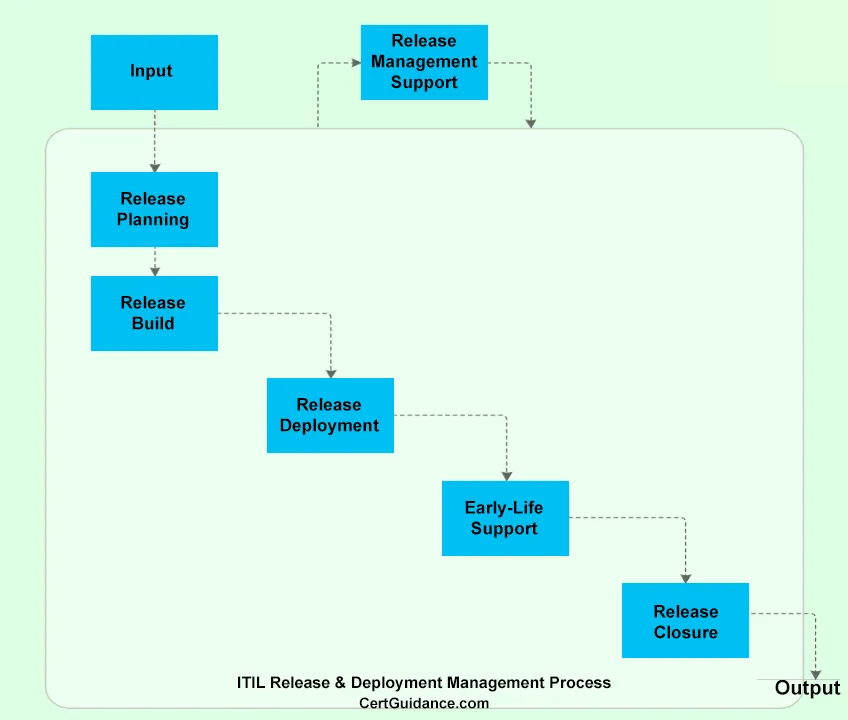
\includegraphics[width=\linewidth]{img/intro_rollout.png}
		\caption{Sottoprocessi di \textit{Release and Deployment Management}\cite{release_deployment_management}}
		\label{fig:intro_rollout}
	\end{figure}

%\section{Utenti e struttura aziendale}\label{sec:struttura_aziendale}
%	
%	Come descritto nel capitolato d'appalto fornito dall'Istituto, il nuovo sistema informatico è rivolto a tutti i dipendenti e ai clienti dei servizi che vengono offerti dalla struttura ospedaliera.
%	
%	Una descrizione più dettagliata degli utenti del servizio e della struttura vengono viene svolta nelle sezioni \ref{ch:servizio_helpdesk} e \ref{sec:utenti}.
	
	
\section{Durata del contratto}
	
	Nonostante la durata totale del contratto sia di nove anni, come descritto nella sezione 5.2 del capitolato fornito dal \proponente, la durata dell'implementazione da parte di \azienda~deve essere completato entro i primi trenta mesi dalla firma del contratto.
	
	Siccome, dal momento della firma del contratto, ci potranno essere cambiamenti \textit{in corsa}, questo documento verrà costantemente aggiornato in maniera da rispecchiare correttamente la corrente pianificazione della fase di \rollout.

%\section{Costo per la fornitura del servizio}
%	\hl{Ha senso scrivere questa sezione? Con che tipo di dati posso riempirla? Che stima faccio?}
	
\section{Penali}

	\azienda~si impegna a rispettare la pianificazione fissata per l'implementazione, delineata in \ref{sec:pianificazione}, e si prende carico delle penali che possono essere imposte in caso di ritardi, o altri eventuali errori, come descritto nel ``\textit{Capitolo 5: Requisiti per i Servizi}'' del capitolato d'appalto fornito dal \proponente.
	
\section{Punti di contatto dell'azienda}

	\azienda~si impegna dare completa disponibilità dei propri contatti con l'\istituto~per qualsiasi comunicazione riguardante il presente documento e il servizio descritto.

	Nella seguente tabella vengono indicati i principali punti di contatto tra \azienda~e l'\istituto.
	\begin{table}[H]
		\renewcommand\arraystretch{2}
		\centering
		\begin{tabular}{|>{\raggedright\arraybackslash}m{3.25cm}|m{4.25cm}|m{4cm}|}
			\hline
			\rowcolor{pantone}
			\multicolumn{1}{|>{\centering\arraybackslash}m{3.25cm}|}{\color{white}\textbf{Ruolo}} &
			\multicolumn{1}{>{\centering\arraybackslash}m{4.25cm}|}{\color{white}\textbf{Nome}} &
			\multicolumn{1}{>{\centering\arraybackslash}m{4cm}|}{\color{white}\textbf{Indirizzo e-mail}}\\
			\hline
			Responsabile privacy			& 	MARIA AMERIO 		& M.AMERIO@\mailazienda		\\\hline
			Responsabile qualità			& 	ANDREA TORCHIO 		& A.TORCHIO@\mailazienda	\\\hline
			Amministratore database			& 	GIOVANNI GAMBA 		& G.GAMBA@\mailazienda		\\\hline
			Responsabile analisi			& 	ROBERTO BARBERO 	& R.BARBERO@\mailazienda	\\\hline
			Responsabile progettazione		& 	ANTONIO PENNA 		& A.PENNA@\mailazienda		\\\hline
			
		\end{tabular}
		\renewcommand\arraystretch{1}
		\caption{Tabella con gli indirizzi e-mail e i ruoli di riferimento}
	\end{table}	
	
	\chapter{Il servizio di Help Desk}\label{ch:servizio_helpdesk}

	L'azienda \azienda, in base agli obiettivi descritti all'interno del capitolato fornito dall'\istituto~Ortopedico Gaetano Pini, stabilisce a sua volta una serie di obiettivi per il \rollout~del nuovo servizio di \helpdesk.
	
	Questi vengono posti con lo scopo di erogare un servizio \textit{misurabile}, assicurando al cliente \textit{alta qualità} e guidando il progetto con \textit{logiche di efficienza ed efficacia}.
	
\section{Lo scopo dell'\helpdesk}\label{sec:scopo_helpdesk}
	
	L'\helpdesk~aziendale è un asset tattico e fondamentale in quanto fornisce un ``\textit{single point of contact}'' (\textit{SPOC}) per gli utenti, ovvero permette di unificare il servizio in un singolo punto centrale.

	Lo scopo principale è quello di fornire aiuto e supporto immediati agli utenti per quanto riguarda i problemi di natura tecnica.
	Questo può fare parte di una infrastruttura informatica aziendale più ampia nella quale sono presenti altri servizi che hanno come scopo creare una struttura organizzata dei servizi volti agli utenti.
	
	Come altri \helpdesk~aziendali, anche quello che viene progettato per l'\istituto~assicura servizi che sono disegnati sulla realtà specifica e dedicati a quest'ultimo.
	
	In Fig. \ref{fig:service-desk-types}~viene rappresentata la struttura generale di un \helpdesk~aziendale, nel quale vi sono un primo, un secondo ed un terzo livello di supporto tecnico all’utente, ciascuno con uno scopo ben preciso:
	% https://www.bmc.com/blogs/support-levels-level-1-level-2-level-3/
	\begin{itemize}[noitemsep]
		\item \textit{\helpdesk~di primo livello}: risoluzione di problemi basilari tramite supporto che non richiede una profonda conoscenza del sistema e dei servizi che lo compongono;
		% Basic help desk resolution and service desk delivery. Support for basic customer issues such as solving usage problems and fulfilling service desk requests that need IT involvement.;
		\item \textit{\helpdesk~di secondo livello}: supporto tecnico che richiede una conoscenza completa del sistema e dei servizi offerti da questo. 
		I problemi che non è possibile risolvere tramite le procedure \textit{prefabbricate} del primo livello, subiscono \textit{escalation} e arrivano al secondo livello;
		% In-depth technical support. Experienced and knowledgeable technicians assess issues and provide solutions for problems that cannot be handled by tier 1.;
		\item \textit{\helpdesk~di terzo livello}: a questo livello tecnici esperti prendono in mano il problema e cercano di risolverlo avendo a loro disposizione tutte le risorse necessarie del sistema.
		% Expert product and service support. Access to the highest technical resources available for problem resolution or new feature creation..
	\end{itemize}

	\begin{figure}[h!]
		\centering
		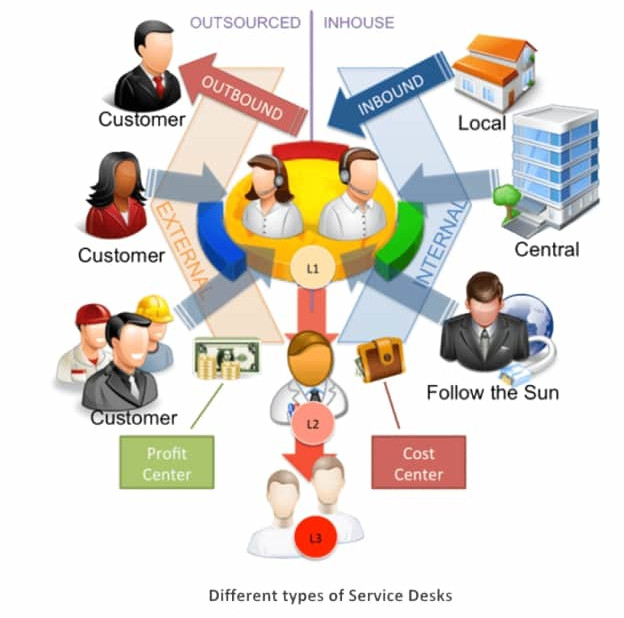
\includegraphics[width=\linewidth]{img/service-desk-types.jpg}
		\caption{``\textit{Service Desk classification}''\cite{service_desk}}
		\label{fig:service-desk-types}
	\end{figure}
	
	\newpage
	
	% https://www.bmc.com/blogs/help-desk-vs-service-desk-whats-difference/
	% The IT help desk is typically seen as more tactical, with the primary goal of helping to quickly resolve end users’ immediate needs and technical issues and incidents. The help desk is reactive in nature, but is expected to be efficient and speedy. The IT help desk can be separate from or part of a larger service desk operation to improve the overall organization’s customer services.

\section{Utenti del servizio}\label{sec:utenti}

	Come descritto nel Capitolato Tecnico dell'istituto, il servizio di \helpdesk~dovrà essere usufruibile da parte di tutto il personale interno dell'azienda e da parte dei clienti, in base alla loro necessità.
	
%	Alcuni esempi di utilizzo da parte degli utenti:
%	\begin{itemize}
%		\item un utente esterno non potrà accedere ai servizi a meno che non sia stato cliente dell'isituto;
%		\item un cliente potrà accedere per vedere solamente i risultati dei servizi di cui ha usufruito;
%		\item gli utenti dell'area amministrativa non potranno avere accesso ad aree come la parte sanitaria e la parte tecnica (server) e viceversa.
%	\end{itemize}

	\subsection{Aree applicative}
	
		\azienda~si impenga, come richiesto dall'\istituto, a implementare i servizi per le seguenti aree applicative:
		\begin{itemize}[noitemsep]
			\item \textit{Area Sanitaria};
			\item \textit{Area Amministrativa};
			\item \textit{Area Direzionale};
			\item \textit{Area Servizi Generali}.
		\end{itemize}
	
		\begin{figure}[h!]
			\centering
			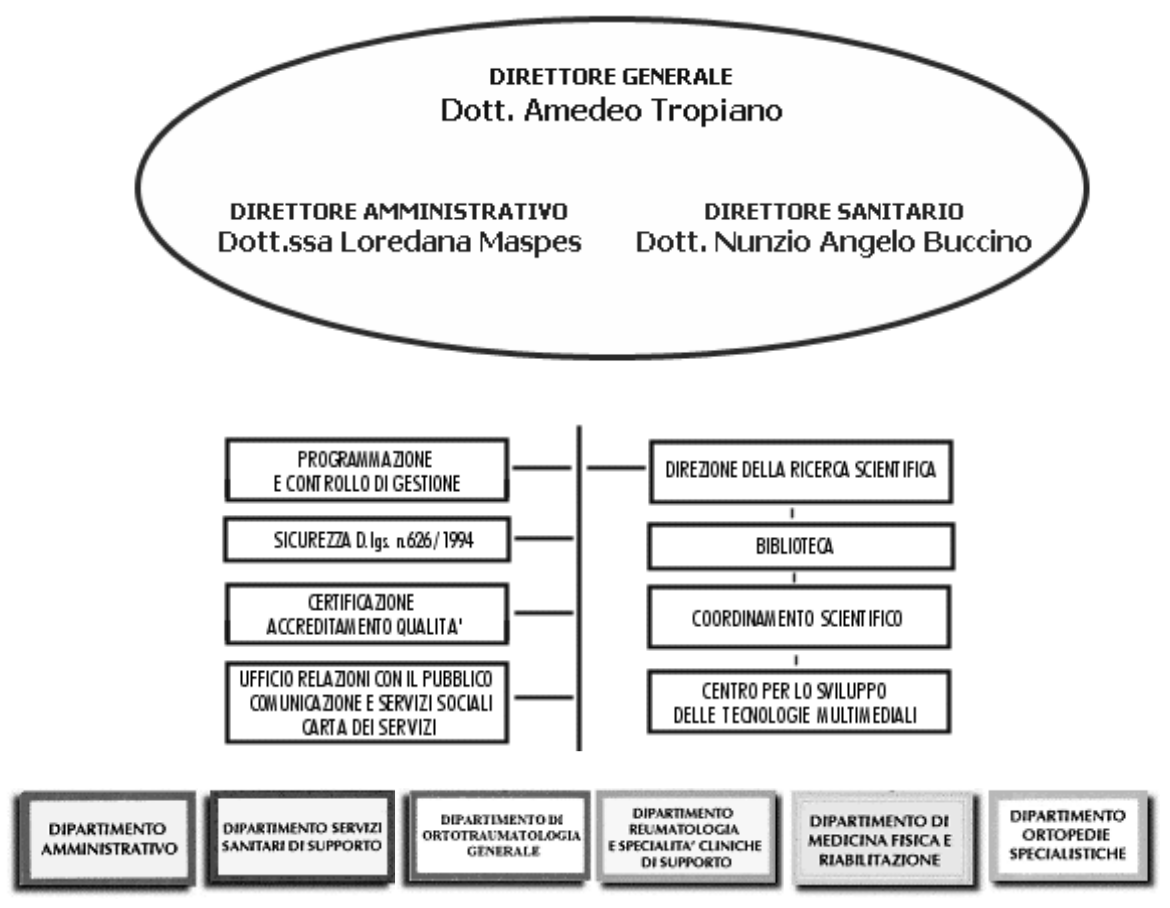
\includegraphics[width=\linewidth]{img/gerarchia.png}
			\caption{Struttura e organizzazione dell'UO Informatico Aziendale}
			\label{fig:gerarchia}
		\end{figure}

		Nel Cap. \ref{ch:implementazione}, viene descritta la modalità di implementazione scelta e come questa avviene per ciascun settore.
		
%\section{Descrizione generale dell’ambiente}\label{sec:ambiente}
%
%	\subsection{Locali fisici dell'ospedale}
%	
%		La descrizione dei locali fisici nei quali è suddiviso l'ospedale si può trovare nel paragrafo 1.1 del capitolato tecnico.

\newpage
\section{Obiettivi del \textit{nuovo} servizio di \helpdesk}\label{sec:obiettivi_helpdesk}

	% Di seguito vengono elencati gli obiettivi che \azienda~ si impegna di rispettare per quanto riguarda il nuovo servizio di \helpdesk, in base a quello che viene richiesto dal \hl{contraente}.
	
	Di seguito vengono elencati gli obiettivi descritti dal \proponente~nel paragrafo 1.2 del capitolato tecnico fornito.
	A ciascuno di questi viene assegnato un identificatore univoco che ne consente una successiva associazione con le attività che \azienda~pianifica di svolgere per portare a termine il progetto.
	
	La classificazione di tali obiettivi permette successivamente di poter verificarne ogettivamente la loro completezza, tramite l'uso di altri parametri, misurandone inoltre la qualità, l'efficacia e l'efficienza.
	
	Gli obiettivi sono dunque presentati in maniera tabulare dove nella prima colonna viene indicato l'identificatore del tipo \textit{IGP\_[NUMERO OBIETTIVO]} (\textit{IGP} come acronimo di \textit{Istituto Gaetano Pini}) e, nella seconda colonna, viene indicato l'obiettivo richiesto.
	
	\newcommand\larghezzacolonnaID{1cm}
	\newcommand\larghezzacolonnaDESC{11cm}

	\begin{table}[H]
		\centering
		\renewcommand\arraystretch{2}
		\begin{tabular}{|>{\raggedright\arraybackslash}m{\larghezzacolonnaID}|m{\larghezzacolonnaDESC}|}
			\hline
			\rowcolor{pantone}
			\multicolumn{1}{|>{\centering\arraybackslash}m{\larghezzacolonnaID}|}{\color{white}\textbf{ID}} &
			\multicolumn{1}{>{\centering\arraybackslash}m{\larghezzacolonnaDESC}|}{\color{white}\textbf{Descrizione}} \\
			\hline
			
			\codiceobiettivo & Ammodernamento organizzativo delle risorse e dei processi, volto al miglioramento della loro efficienza, all’interscambio informativo ed al governo dell’attività aziendale.
			\\\hline
			
			\codiceobiettivo & \vfill Razionalizzazione del sistema informatico e del servizio. \vfill
			\\\hline
			
			\codiceobiettivo & Consolidamento dei sistemi (hw, sw) per avere maggiore facilità di gestione.
			\\\hline
			
			\codiceobiettivo & Riprogettazione del sistema ed evoluzione tecnologica dei componenti dove più obsoleti.
			\\\hline
			
			\codiceobiettivo & Riprogettazione dei servizi generali di continuità, sicurezza, ecc. al fine di avere una architettura più stabile e trasversale ai diversi sistemi.
			\\\hline
						
			\codiceobiettivo & Presa in carico del sistema informativo sia per nuove componenti offerte sia per l’esistente; è lasciata facoltà all’offerente di mantenere gli attuali sistemi, ottimizzandone il funzionamento rispetto ai livelli di servizio richiesti, oppure di procedere alla sostituzione degli stessi. Per quest’ultimo aspetto, l’offerente dovrà farsi carico della completa migrazione delle informazioni gestite.
			\\\hline
					
		\end{tabular}
		\renewcommand\arraystretch{1}
		\caption{Lista obiettivi del nuovo \helpdesk~(pt. 1)}
	\end{table}	

	\begin{table}[H]
		\centering
		\renewcommand\arraystretch{2}
		\begin{tabular}{|>{\raggedright\arraybackslash}m{2cm}|m{10cm}|}
			\hline
			\rowcolor{pantone}
			\multicolumn{1}{|>{\centering\arraybackslash}m{2cm}|}{\color{white}\textbf{ID}} &
			\multicolumn{1}{>{\centering\arraybackslash}m{10cm}|}{\color{white}\textbf{Descrizione}} \\\hline
			
			\codiceobiettivo & Standardizzazione degli ambienti, con adeguamento alle principali normative e standard correnti, assicurando al contempo il mantenimento delle specificità dell’Istituto.
			\\\hline
			
			\codiceobiettivo & Impulso alla dematerializzazione dei documenti scambiati in Istituto e dall’Istituto, con conseguente risparmio sia di materiali (carta) che di tempo.
			\\\hline
			
			\codiceobiettivo & Supporto nei processi di riorganizzazione che l’Istituto che mettendo in atto, quali, ad esempio non esaustivo:
			\begin{itemize}[noitemsep]
				\item passaggio completo a controllo di gestione e budgeting;
				\item unificazione rete imaging;
				\item collegamento tra flussi dei sistemi gestionali sanitari e processi clinici e diagnostici.
			\end{itemize}
			\\\hline
		
			\codiceobiettivo & Progettazione e fornitura di sistemi applicativi che possano essere utilizzati quali base per la successiva introduzione di nuovi servizi innovativi; inoltre, disponibilità a realizzare sperimentazioni di nuovi sistemi.
			\\\hline
			
			\codiceobiettivo & Organizzazione del servizio con interfacce univoche verso la direzione e verso gli utenti.
			\\\hline
			
			\codiceobiettivo & Consolidamento dei servizi di gestione e assistenza, attualmente dispersi tra diversi fornitori, per evitare la frammentazione delle responsabilità.
			\\\hline
			
			\codiceobiettivo & Disponibilità di strumenti di controllo dei livelli di servizio forniti.
			\\\hline
			
			\codiceobiettivo & Disponibilità di strumenti per la registrazione, l’analisi ed il tracciamento delle richieste dell’utenza.
			\\\hline
			
			\codiceobiettivo & La manutenzione, assistenza e gestione dei sistemi attualmente in uso e che si intende mantenere nell’architettura globale, assicurandone l’evoluzione nei prossimi 9 anni.
			\\\hline
			
		\end{tabular}
		\renewcommand\arraystretch{1}
		\caption{Lista obiettivi del nuovo \helpdesk~(pt. 2)}
	\end{table}	
	\begin{table}[H]
		\centering
		\renewcommand\arraystretch{2}
		\begin{tabular}{|>{\raggedright\arraybackslash}m{2cm}|m{10cm}|}
			\hline
			\rowcolor{pantone}
			\multicolumn{1}{|>{\centering\arraybackslash}m{2cm}|}{\color{white}\textbf{ID}} &
			\multicolumn{1}{>{\centering\arraybackslash}m{10cm}|}{\color{white}\textbf{Descrizione}} \\\hline
			
			\codiceobiettivo & La fornitura di nuovi sistemi invece di quelli attualmente in uso e che si intende sostituire, evidenziando il razionale della sostituzione e i vantaggi introdotti con le nuove soluzioni.
			\\\hline
			
			\codiceobiettivo & L’attuazione di un progetto organizzativo, completo di attività di BPR, in grado di supportare efficacemente l’adozione della piattaforma applicativa proposta, tenendo conto delle esigenze e delle specificità dell’Istituto.
			\\\hline
			
			\codiceobiettivo & La fornitura di nuovi sistemi che integrano e si aggiungono a quelli già in uso sia in forma definitiva che di sperimentazione.
			\\\hline
			
			\codiceobiettivo & L’eventuale progettazione e realizzazione dei lavori per la riorganizzazione dei locali CED. Sarà cura dell’offerente definire quali sistemi mantenere nel CED dell’Istituto e quali ospitare presso un proprio centro esterno di servizio adeguatamente collegato per via telematica a spese dell’offerente stesso.
			\\\hline
			
			\codiceobiettivo & La sperimentazione di soluzioni innovative.
			\\\hline
			
			\codiceobiettivo & Tutti i servizi di gestione, manutenzione ed assistenza di tutti i sistemi di cui ai punti precedenti, l’organizzazione del Centro di Gestione Integrato ed i servizi di supporto professionale (direzionale, gestione personale).
			\\\hline
			
			\codiceobiettivo & Evidenzi le capacità progettuali e le competenze dell’offerente descrivendo:
			\begin{itemize}[noitemsep]
				\item un progetto tecnico di proposta per l’Integrazione della Rete Radiologica;
				\item le soluzioni disponibili e le proposte dell’offerente riguardo ai progetti di sperimentazione ed innovazione descritti in dettaglio successivamente o proposti dall’offerente stesso.
			\end{itemize}
			\\\hline
	
		\end{tabular}
		\renewcommand\arraystretch{1}
		\caption{Lista obiettivi del nuovo \helpdesk~(pt. 3)}
	\end{table}	

	\newpage
	\subsection{Business Process Re-engineering (BPR)}\label{sec:desc_bpr}
		
		Per ``\textit{Business Process Re-engineering}'' (in italiano ``\textit{riprogettazione dei processi aziendali}'') si intende un intervento organizzativo di profonda revisione dei procedimenti operativi che non risultano più adeguati alle necessità aziendali.
		Come ciascun altro processo, anche quelli di BRP richiedono un \textit{input} e, dopo averlo elaborato, restituiranno un determinato \textit{output}.
		
		Nel caso specifico dell'\istituto, come richiesto da capitolato, è necessario rivedere e correggere l'attuale sistema gerarchico, implementando processi aziendali moderni e adatti al nuovo sistema informatico che \azienda~si è proposta di progettare.
		Da un modello \textit{gerarchico-funzionale} l'Istituto vuole passare ad un modello per processi, caratterizzato da una maggiore integrazione con il sistema di \helpdesk.
	
		\begin{figure}[H]
			\centering
			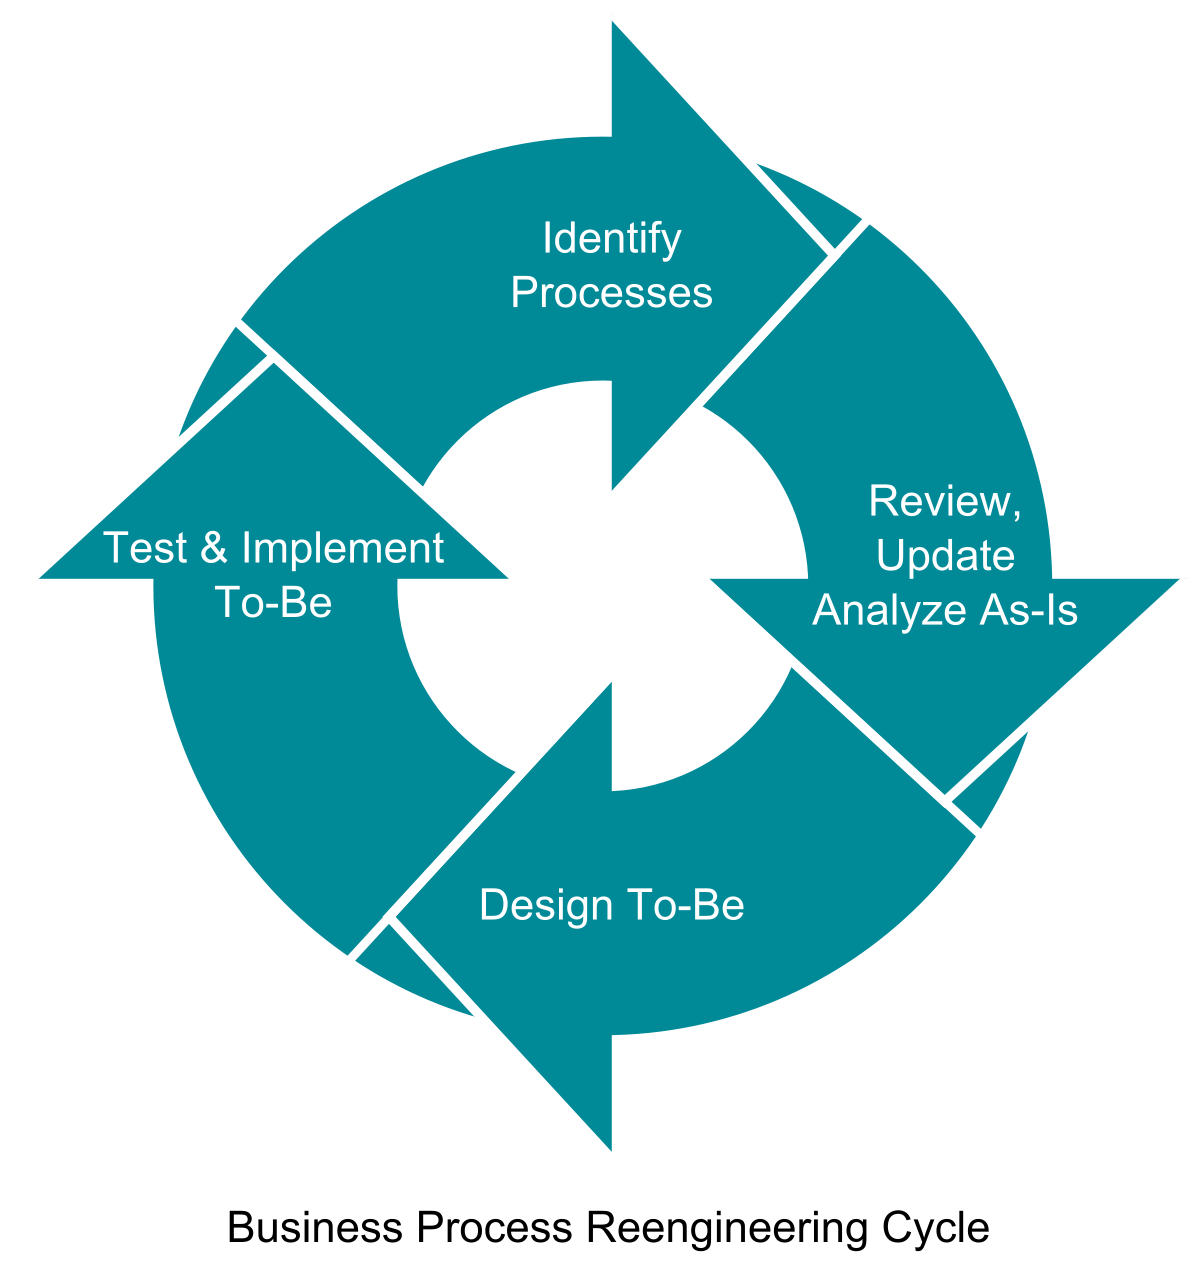
\includegraphics[width=\linewidth-2cm]{img/bpr}
			\caption{``\textit{Business process re-engineering cycle}''\cite{bpr}}
			\label{fig:bpr}
		\end{figure}
	
		L'attività di BPR può essere suddivisa in quattro fasi, come in Fig.~\ref{fig:bpr}:
		\begin{enumerate}
			\item \textit{Identificazione dei processi} (\textit{Identify Processes}): durante questa fase è necessario identificare i processi esistenti (\textit{as-is}) per avere le informazioni di base da cui partire;
			\item \textit{Revisione, aggiornamento e analisi dell’as-is} (Review, Update, Analyze As-is): in questa fase è necessario analizzare in profondità i processi identificati, allo scopo di avere più informazioni possibili;
			\item \textit{Design to-be}: in questa fase vengono progettati i nuovi processi, seguendo le linee guida e gli obiettivi del \proponente;
			\item \textit{Test e implementazione del to-be} (Test \& Implement To-Be): in quest’ultima fase i processi vengono testati ed effettivamente implementati nella realtà aziendale del \proponente.
		\end{enumerate}

		Per l'implementazione da parte di \azienda~si rimanda il lettore al paragrafo \ref{subsec:bpr_implmentation}.    
  	\chapter{\textit{Deployment} del nuovo sistema informatico}\label{ch:implementazione}

% In questa sezione verranno descritte le dinamiche di gestione per l’implementazione della soluzione, identificando le attività principali e suddividendole in compiti (tasks).

In questo capitolo viene descritta la pianificazione per la gestione del deployment della soluzione proposta da \azienda.


Vengono quindi individuate le attività principali e, per ciascuna di queste, vengono definiti dei \textit{task}.
Tali attività sono strettamente collegate con gli obiettivi presenti nella Sez. \ref{sec:obiettivi_helpdesk}~in quanto sono svolte al fine di soddisfare questi ultimi.

\section{Descrizione dell’implementazione}\label{sec:desc_implementazione}

	Per la transizione dal sistema informatico corrente a quello nuovo, \azienda~ha deciso di utilizzare totalmente il tempo di sei mesi fornito dal proponente.
	
	Dopo un'attenta analisi, \azienda~ha optato di effettuare un \rollout~con la tipologia \textit{Verticale}, scartando dnuque quella \textit{Orizzontale}.
	Questo in quanto, vista la suddivisione dell'azienda ospedaliera in multipli reparti, che possiamo definire modulari, risulta più conveniente e meno propenso ad errori, permettendo inoltre di adattare e testare facilmente il nuovo sistema in corso d'opera.
	
	\begin{figure}[h!]
		\centering
		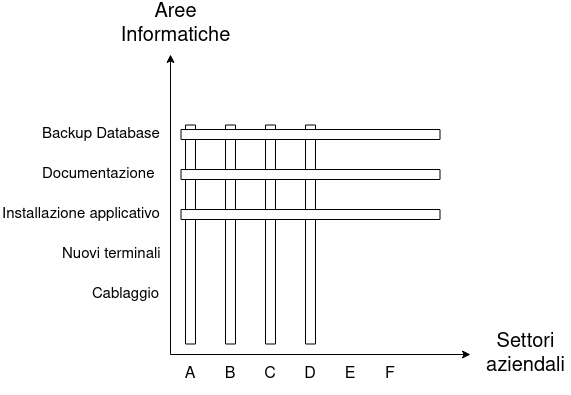
\includegraphics[width=\linewidth]{img/implementazione.png}
		\caption{Implementazione verticale \textit{vs} implementazione orizzontale}
		\label{fig:implementazione}
	\end{figure}

	In Fig. \ref{fig:implementazione}~è possibile vedere rappresentata in un grafico la differenza principale tra implementazione verticale, che appunto viene svolta in successione per ciascun settore aziendale, e quella orizzontale, che prevede implementare la feature in un unico momento in ciascun settore.

\newpage
\subsection{Implementazione Orizzontale}

	Un'implementazione orizzontale consiste nell'effettuare il passaggio da un sistema ad un altro in tutta l'azienda in una singola transizione.
	Questo approccio porta alcuni vantaggi, quali:
	\begin{itemize}[noitemsep]
		\renewcommand\labelitemi{--}
		\item tempo totale di transizione e implementazione più brevi;
		\item non ci possono essere due sistemi diversi utilizzati contemporaneamente all’interno dell’azienda;
		\item non sono presenti dispositivi che fungono da traduttori tra un sistema e un altro;
		\item è possibile concentrare le risorse esclusivamente per l'implementazione del nuovo sistema e non alla creazione di interfacce o fix per il sistema uscente;
		\item minori costi complessivi, essendo che il vecchio sistema viene dismesso più in fretta.
	\end{itemize}
	
	Tuttavia, sono presenti anche alcuni svantaggi, come ad esempio:
	\begin{itemize}[noitemsep]
		\renewcommand\labelitemi{--}
%		\item difficoltà nell'esecuzione dei test prima del passaggio nell'ambiente di produzione;
		\item impossibilità di eseguire un roll-back affidabile nel lungo periodo, dopo la dismissione del vecchio sistema;
		\item cambiamento improvviso del workflow lavorativo dei dipendenti e una conseguente diminuzione temporanea di produttività.
	\end{itemize}

\subsection{Implementazione Verticale}

	L'implementazione verticale è un approccio che effettua una transizione graduale ed uniforme del sistema all'interno dell'azienda.
	
	Per questa tipologia di \rollout~i vantaggi sono:
	\begin{itemize}[noitemsep]
		\renewcommand\labelitemi{--}
		\item un adattamento più chiaro e veloce al nuovo sistema informatico;
		\item problemi e difficoltà di implementazione possono essere scoperte prima che tutta l'azienda ne sia affetta, ma solamente una singola area, e quindi risolti in maniera graduale;
		\item la loro produttività resta inalterata grazie al cambio graduale;
	\end{itemize}

	Come per l'implementazione orizzontale, anche quella verticale presenta alcuni svantaggi, quali:
	\begin{itemize}[noitemsep]
		\renewcommand\labelitemi{--}
		\item costi di implementazione più alti a causa, tra cui, della coesistenza parziale di due sistemi;
		\item presenza di interfacce per la comunicazione tra un sistema e un altro;
		\item periodo prolungato di formazione;
		\item difficoltà di integrazione dei due sistemi.
	\end{itemize}

\section{Fasi dell'implementazione}

	Dopo un'attenta lettura del capitolato, le fasi definite per l'implementazione del nuovo sistema sono:
	\begin{enumerate}
		\item \textbf{Definizione del nuovo \helpdesk}
			\begin{itemize}[noitemsep]
				\renewcommand\labelitemi{--}
				\item Identificazione, discussione e approvazione dei moduli;
				\item Identificazione delle eventuali estensioni al progetto;
				\item Identificazione delle eventuali personalizzazioni al progetto;
				\item Identificazione dei requisiti della soluzione e dei criteri di soddisfacimento.
			\end{itemize}
			
		\item \textbf{Sviluppo del nuovo \helpdesk}
			\begin{itemize}[noitemsep]
				\renewcommand\labelitemi{--}
				\item Realizzazione di mockup e PoC dei servizi principali del nuovo sistema;
				\item Definizione di eventuali estensioni a tali servizi;
				\item Implementazione delle estensioni richieste;
				\item Realizzazione e presentazione di un prototipo;
				\item Completamento del prototipo e test;
				\item Realizzazione di documentazione tecnica ed altro materiale per gli utenti.
			\end{itemize}
			
		\newpage
		\item \textbf{Installazione per area}
			\begin{itemize}[noitemsep]
				\renewcommand\labelitemi{--}
				\item Installazione delle soluzioni su ambienti di produzione, di sviluppo e di test per ciascuna delle aree dell'istituto definite nel capitolato d'appalto;
				\item Configurazione delle soluzioni in base alle necessità definite precedentemente;
				\item Impostazione dei profili utente e assegnazione dei privilegi;
				\item Importazione dei dati necessari al funzionamento della nuova soluzione.
			\end{itemize}
		
		\item \textbf{Formazione dei dipendenti dell'\istituto~sul nuovo sistema}
			\begin{itemize}[noitemsep]
				\renewcommand\labelitemi{--}
				\item Affiancamento di \azienda~al \proponente~per fornire formazione agli utenti del nuovo sistema;
				\item Adeguamento della documentazione e dei manuali utente.
			\end{itemize}
		
		\item \textbf{Installazione per area del nuovo sistema in produzione}
			\begin{itemize}[noitemsep]
				\renewcommand\labelitemi{--}
				\item Per ciascuna area, l'\istituto, dopo aver validato che siano stati implementati tutti i requisiti, autorizza \azienda~a procedere al passaggio dal vecchio al nuovo sistema;
				\item Trasferimento dei dati dal vecchio al nuovo sistema;
				\item Freeze del vecchio sistema in caso di \rollback;
			\end{itemize}
		
		\item \textbf{Affiancamento dei dipendenti in vista della riconsegna}
			\begin{itemize}[noitemsep]
				\renewcommand\labelitemi{--}
				\item Affiancamento da parte di \azienda~verso l'\istituto~nel primo periodo di utilizzo del nuovo sistema;
				\item Eventuale perfezionamento della documentazione;
				\item Risoluzione di eventuali bug e perfezionamento del sistema (tramite piccole modifiche);
				\item Identificazione e risoluzione di incidenti e problemi;
				\item Successivamente, supporto da parte di \azienda~tramite il proprio Service Desk.
			\end{itemize}
		
	\end{enumerate}

	Le fasi numero tre, ``\textit{Installazione per area}'', e cinque, ``\textit{Go-live del nuovo sistema per area}'', rappresentano l'installazione e la messa in produzione del sistema in base a ciascuna delle aree ospedaliere presenti nel capitolato fornito dal \proponente.
	Questo in quanto viene effettuato un \rollout~con implementazione verticale, come spiegato in \ref{sec:desc_implementazione}.
	
	\subsection{Presa in carico del progetto}
	
		Come specificato nel capitolato fornito dall'\istituto, il \proponente~desidera passare da una fornitura con service provider multipli ad una fornitura di tipo ``\textit{sole provider}''.
	
		\azienda~si impegna dunque a prendere in carico la gestione di tutti i contratti esistenti alla data di aggiudicazione dell'appalto, contattando gli attuali fornitori e terminando i servizi in essere.
		Avvisare gli attuali fornitori è essenziale per una regolare e corretta presa in carico.
		
		In caso di irregolarità o incomprensioni, \azienda~avvertirà il Coordinatore di Progetto, allo scopo di prendere una decisione per risolvere la situazione.
	
	% TODO scrivere altro?
	\subsection{Riconsegna del progetto}
	
		Come descritto da capitolato, \azienda si impegna a riconsegnare il progetto completo dopo nove anni passati dalla presa in carico.

		Verranno quindi consegnate le credenziali di accesso al sistema, tutta la documentazione prodotta, tutti i sistemi hardware e software comprati e prodotti durante la durata del progetto e tutte le risorse che erano state fornite ad \azienda~con lo scopo di completare il progetto descritto nel capitolato d'appalto.

\section{Attività principali}\label{sec:attivita_principali}

	In questa sezione vengono analizzate con maggiore attenzione alcune delle attività principali della fase di implementazione.
	Per ciascuna di queste vi sono cinque indicatori:
	\begin{itemize}[noitemsep]
		\renewcommand\labelitemi{--}

		\item \textit{Input}: i dati e le informazioni che vengono dati in input all'attività in maniera che questa funzioni correttamente;

		\item \textit{Deliverable} (o \textit{Output}): quello che viene prodotto dall'attività, potrebbero essere oggetti materiali o artefatti digitali;

		\item \textit{Risorse}: risorse necessarie dall'attività per trasformare l'input nell'output;

		\item \textit{Criteri di accettazione}: criteri, accordati tra \azienda~e proponente, che dicono quando un'attività è stata conclusa con successo; 

		\item \textit{Responsabili}: ruoli responsabili del corretto svolgimento dell'attività.
		
	\end{itemize}

	Inoltre, quando necessario, l'attività verrà suddivisa in compiti (tasks) aventi maggiore granularità.
	Successivamente, nella Sez. \ref{sec:pianificazione}, viene presentata una pianificazione di tali attività.
	
	Le attività di seguito presentate sono strettamente correlate con gli obiettivi elencati in \ref{sec:obiettivi_helpdesk}.
	
%	\newpage
	\subsection{Implementazione della nuova \textit{BPR}}\label{subsec:bpr_implmentation}

		L'attività di BPR tratta una profonda revisione dei processi aziendali, che, come spiegato in \ref{sec:desc_bpr}, si intende un intervento organizzativo di \textit{profonda revisione} dei procedimenti operativi.
		
		Tale attività può cominciare da subito in quanto prevede una lunga e profonda analisi del modello attuale dell'istituto
		
		\begin{itemize}[noitemsep]
			\renewcommand\labelitemi{--}
			\item \textbf{Input}: manuali e osservazioni del modello gerarchico attualmente in uso dall'azienda, ovvero analisi della situazione \textit{as-is};
			\item \textbf{Deliverable}: documento che descrive i nuovi processi creati in base alle necessità aziendali del proponente e documento che descrive le attività necessarie alla transizione dalla struttura gerarchica al nuovo sistema tramite BPR e l'implementazione di questo;
			%, documento che descrive l'attuale modello gerarchico funzionale dell'istituto situazione attuale dei processi aziendali;
			\item \textbf{Risorse}: personale esperto in processi aziendali di \azienda~e personale dell'istituto che si occupa dell'organizzazione del modello gerarchico, ciascuno dotato di un proprio computer, adetto all'analisi dell'attuale modello e alla stesura dei nuovi processi aziendali;
			\item \textbf{Criteri di accettazione}: accettazione da parte del proponente dei nuovi processi stilati;
			\item \textbf{Responsabili}: analisti con conoscenza di processi aziendali.
		\end{itemize}
	
		\textbf{Tasks:}
		\begin{enumerate}[noitemsep]
			\item analisi dell'attuale modo di lavoro;
			\item stesura dei nuovi processi;
			\item approvazione di tali processi da parte del proponente.
		\end{enumerate}
	
		Gli obiettivi che questa attività è volta a soddisfare sono:
		\begin{itemize}[noitemsep]
			\renewcommand\labelitemi{--}
			\item {\color{pantone}IGP\_\ref{igp:1}}
			\item {\color{pantone}IGP\_\ref{igp:7}}
			\item {\color{pantone}IGP\_\ref{igp:8}}
			\item {\color{pantone}IGP\_\ref{igp:9}}
		\end{itemize}

%	\newpage
	\subsection{Scrittura della documentazione relativa al progetto}
	
		Come per l'attività precedente, anche quella riguardante la documentazione a una durata che parte dall'inizio del progetto fino alla sua conclusione.
		
		Avere una documentazione aggiornata e ben organizzata è inoltre alla base delle richieste da rispettare per perseguire certificazioni di standard, come richiesto appunto dall'\istituto~in {\color{pantone}IGP\_\ref{igp:7}}.
		
		\begin{itemize}[noitemsep]
			\renewcommand\labelitemi{--}
			\item \textbf{Input}: intero archivio della documentazione attuale riguardante il sistema informatico attualmente in uso e il sistema gerarchico;
			\item \textbf{Deliverable}: vengono forniti in output tutti i documenti riguardanti il progetto e la sua evoluzione;
			\item \textbf{Risorse}: per questa attività ciascuna delle persone coinvolte nel progetto dovrà dedicare tempo per documentare ciò che ha svolto;
			\item \textbf{Criteri di accettazione}: criteri quali chiarezza nella lettura e correttezza con quanto svolto verranno usati per validare il documento;
			\item \textbf{Responsabili}: i manager di ciascun gruppo saranno responsabili per la qualità della documentazione prodotta.
		\end{itemize}
		
		\textbf{Tasks:}
		\begin{enumerate}[noitemsep]
			\item ciascun dipendente pianifica le attività che deve svolgere;
			\item durante e dopo aver svolto tale attività, i dipendenti dovranno usare template forniti da \azienda~e concordati con l'\istituto, per documentare quanto svolto;
			\item riunioni a cadenza settimanale o bisettimanale, in base alle attività svolte, verranno usate per revisionare i documenti ed accettarli.
		\end{enumerate}
	
		Gli obiettivi che questa attività è volta a soddisfare sono:
		\begin{itemize}[noitemsep]
			\renewcommand\labelitemi{--}
			\item {\color{pantone}IGP\_\ref{igp:1}}
			\item {\color{pantone}IGP\_\ref{igp:7}}
			\item {\color{pantone}IGP\_\ref{igp:8}}
			\item {\color{pantone}IGP\_\ref{igp:9}}
			\item {\color{pantone}IGP\_\ref{igp:15}}
			\item {\color{pantone}IGP\_\ref{igp:17}}
		\end{itemize}

%	\newpage
	\subsection{\textit{Hand-off} dei sistemi ed erogazione dei servizi esistenti}
		
		La presa in carico dei sistemi esistenti da parte dell'offerente implica l'impegno di \azienda~ad erogare senza interuzioni i servizi che i precedenti fornitori offrivano.
		
		\begin{itemize}[noitemsep]
			\renewcommand\labelitemi{--}
			\item \textbf{Input}: documentazione e strumentazione relative a tutti i servizi attualmente in uso;
			\item \textbf{Deliverable}: continuativa erogazione dei servizi esistenti;
			\item \textbf{Risorse}: personale tecnico dell'istituto che possa spiegare e direzionare gli esperti di \azienda~per un corretto hand-off;
			\item \textbf{Criteri di accettazione}: erogazione dei servizi attuali senza interruzione;
			\item \textbf{Responsabili}: il responsabile della progettazione sarà colui che pianificherà la transizione in maniera che questa avvenga senza interruzioni.
		\end{itemize}
		
		\textbf{Tasks:}
		\begin{enumerate}[noitemsep]
			\item meeting di presentazione da parte dei tecnici di \azienda~e istituto nel quale vengono spiegati i sistemi attualmente in uso e quali servizi vengono erogati;
			\item ottenimento da parte dei tecnici di \azienda~delle credenziali e dei permessi necessari per poter accedere a tali sistemi e garantire una corretta erogazione;
			\item analisi delle logiche e delle modalità di erogazione dei servizi in uso;
			\item analisi e test dei servizi esistenti da parte dei tecnici di \azienda~insieme ai responsabili del proponente per assigurarsi di una corretta erogazione.
		\end{enumerate}
	
		Gli obiettivi che questa attività è volta a soddisfare sono:
		\begin{itemize}[noitemsep]
			\renewcommand\labelitemi{--}
			\item {\color{pantone}IGP\_\ref{igp:4}}
			\item {\color{pantone}IGP\_\ref{igp:5}}
			\item {\color{pantone}IGP\_\ref{igp:6}}
			\item {\color{pantone}IGP\_\ref{igp:12}}
			\item {\color{pantone}IGP\_\ref{igp:15}}
			\item {\color{pantone}IGP\_\ref{igp:16}}
			\item {\color{pantone}IGP\_\ref{igp:18}}
			\item {\color{pantone}IGP\_\ref{igp:19}}
		\end{itemize}

%	\newpage
	\subsection{Presa in carico postazioni di lavoro}
	
		Come elencato nel capitolato tecnico fornito dall'\istituto, le postazioni di lavoro dei dipendenti attualmente presenti sono molto diverse in quanto provvengono da fornitori diversi e dunque sono di marche e anni di acquisto diversi.
		Per certe postazioni alcuni di questi dati non sono disponibili.
		Tali contraddizioni sono la causa di un processo di \textit{Service Asset} e \textit{Configuration Management} svolti in maniera non ottimale.
		
		\azienda, come richiesto dal proponente, prende in carica la gestione di tali postazioni e garantisce di risolvere le problematiche riguardo il magazzino e di incongruenze nell'hardware.
		A tale scopo verrà istutuito un processo per controllare regolarmente le postazioni di lavoro.
		\azienda~si impegna inoltre di creare un sistema di magazzino in maniera da monitorare la presenza dei pezzi di ricambio con una granularità congrua alle necessità dell'\istituto.
		
		Attività di riorganizzazione come questa aiutano l'\istituto~a diventare eleggibile per certificazioni di standard e normative nazionali ed internazionali, come richiesto nell'obiettivo {\color{pantone}IGP\_\ref{igp:7}}.
		
		All'interno di questa attività vengono inclusi anche strumenti come stampanti e altro hardware che funge da periferiche per i computer.
		Come per i computer, anche tali dispositivi verranno registrati in magazzino e verranno forniti pezzi di ricambio, quando possibile.
		
		\begin{itemize}[noitemsep]
			\renewcommand\labelitemi{--}
			\item \textbf{Input}: lista completa dell'hardware presente all'interno dell'istituto, credenziali di accesso ai sistemi, privilegi necessari per poter installare nuovo hardware;
			\item \textbf{Deliverable}: sistemi uniformi in tutto l'istituto e un sistema di stoccaggio che permette di tracciare i pezzi in uso e gli eventuali pezzi di ricambio;
			\item \textbf{Risorse}: personale tecnico dell'istututo che indichi dove sono presenti i computer e altro hardware attualmente in uso;
			\item \textbf{Criteri di accettazione}: corretta integrazione dei nuovi computer e adeguata potenza in base alle necessità dei dipendenti e delle funzioni che devono svolgere;
			\item \textbf{Responsabili}: il responsabile alla progettazione e il responsabile alla privacy saranno incaricati della supervisione e della corretta esecuzione di tale attività.
		\end{itemize}
		
		\textbf{Tasks:}
		\begin{enumerate}[noitemsep]
			\item identificazione delle attuali postazioni di lavoro, e altro hardware, da sostituire;
			\item stipulazione di un contratto per l'acquisto di nuovo hardware, possibilmente con un grande magazzino o una casa madre;
			\item catalogazione nel magazzino e installazione del nuovo hardware;
			\item test e benchmark dei nuovi sistemi.
		\end{enumerate}

		Gli obiettivi che questa attività è volta a soddisfare sono:
		\begin{itemize}[noitemsep]
			\renewcommand\labelitemi{--}
			\item {\color{pantone}IGP\_\ref{igp:2}}
			\item {\color{pantone}IGP\_\ref{igp:3}}
			\item {\color{pantone}IGP\_\ref{igp:4}}
			\item {\color{pantone}IGP\_\ref{igp:6}}
			\item {\color{pantone}IGP\_\ref{igp:7}}
			\item {\color{pantone}IGP\_\ref{igp:11}}
			\item {\color{pantone}IGP\_\ref{igp:18}}
		\end{itemize}

%	\newpage
	\subsection{Revisione cablaggio e architettura di rete}\label{subsec:revisione_rete}
	
		Come descritto all'interno del capitolato fornito dall'\istituto, l'attuale architettura di rete presenta alcune problematiche, quali, ad esempio, tratti a bassa velocità, tratti che bypassano il centro stella, per collegarsi direttamente al centro elaborazione dati (o \textit{CED}).

		L'attuale organizzazione della rete ospedaliera rende tale centro stella un \textit{single point of failure} che mette a repentaglio l'intero sistema.
		Questo dovuto al fatto che non ci sono \textit{failover}, ovvero non vi sono sistemi secondari che possono subentrare in caso di malfunzionamenti.
		
		\azienda~si impegna dunque a riformare tale rete in maniera da renderla solida e sicura, assicurando dunque che non vi siano points of failure fatali e che, anche in caso di eventuali fallimenti, i dipendenti non si accorgano del downtime.
	
		Per fare ciò, può essere necessario l'acquisto di nuovi server o apparati di rete, anche dello stesso marchio e modello in maniera da facilitarne la manutenzione.
	
		\begin{itemize}[noitemsep]
			\renewcommand\labelitemi{--}
			\item \textbf{Input}: mappa della rete attuale, accesso alla strumentazione e all'hardware che forma la rete;
			\item \textbf{Deliverable}: una rete ristrutturata e solida insieme alla documentazione che ne spiega il partizionamento e il piano di indirizzamento; 
			\item \textbf{Risorse}: analisti e progettisti di rete e nuovo hardware;
			\item \textbf{Criteri di accettazione}: la nuova rete deve soddisfare tutti i requisiti del proponente per l'interconnessione dei computer e altro hardware. Tali requisiti vengono validati tramite test sulla ridondanza e sulle funzionalità di rete;
			\item \textbf{Responsabili}: progettisti di rete.
		\end{itemize}
		
		\textbf{Tasks:}
		\begin{enumerate}[noitemsep]
			\item analisi della rete attuale da parte di \azienda;
			\item stesura di un documento piano di indirizzamento IP e di partizionamento della rete;
			\item implementazione della nuova rete con eventuali nuovi server ed altri apparati di rete;
			\item convalida del nuovo sistema tramite test che ne possano verificare il corretto funzionamento e ridondanza.
		\end{enumerate}

		Gli obiettivi che questa attività è volta a soddisfare sono:
		\begin{itemize}[noitemsep]
			\renewcommand\labelitemi{--}
			\item {\color{pantone}IGP\_\ref{igp:2}}
			\item {\color{pantone}IGP\_\ref{igp:3}}
			\item {\color{pantone}IGP\_\ref{igp:4}}
			\item {\color{pantone}IGP\_\ref{igp:5}}
			\item {\color{pantone}IGP\_\ref{igp:6}}
			\item {\color{pantone}IGP\_\ref{igp:15}}
			\item {\color{pantone}IGP\_\ref{igp:16}}
		\end{itemize}
	
%	\newpage
	\subsection{Revisione del \textit{Centro Elaborazione Dati} (\textit{CED})}
		
		\azienda, vista la necessità di riprogettare il Centro Elaborazione Dati (o \textit{CED}) dell'\istituto, ha scelto di optare per una soluzione ibrida tra server in cloud e server \textit{in loco}, acquistati e tenuti localmente all'interno della struttura.
		
		Tale scelta è stata fatta in quanto una corretta integrazione tra cloud e locale facilita la manutenzione di operazioni come ad esempio i backup automatizzati e permette di avere meno possibili \textit{points of failure}, come accennato in \ref{subsec:revisione_rete} per il centro stella della rete.
		
		Il principale obiettivo che va ad essere soddisfatto da questa attività è {\color{pantone}IGP\_\ref{igp:19}}, nel quale l'\istituto~esprime il bisogno di una riorganizzazione dei locali CED presenti all'interno del sistema.
		
		\begin{itemize}[noitemsep]
			\renewcommand\labelitemi{--}
			\item \textbf{Input}: documentazione necessaria sui servizi attuali del CED, hardware e software (inclusi di codice sorgente ove presente) che compongono il CED, obiettivi e requisiti del nuovo CED;
			\item \textbf{Deliverable}: un nuovo CED aggiornato e \textit{ad-hoc} creato in base alle necessità dell'\istituto;
			\item \textbf{Risorse}: personale tecnico dell'\istituto~che affiancherà i dipendenti di \azienda~nella creazione del nuovo CED;
			\item \textbf{Criteri di accettazione}: per tale attività i criteri rappresentano i test di accettazione finali che stabiliranno se il nuovo CED rispetta tutti gli obiettivi e le richieste fatte dagli stakeholders;
			\item \textbf{Responsabili}: il responsabile della progettazione del nuovo sistema si occuperà di controllare che il proseguimento del lavoro sia in linea con quello che viene richiesto dall'istituto.
		\end{itemize}
		
		\textbf{Tasks:}
		\begin{enumerate}[noitemsep]
			\item presa in carico del sistema \textit{as-is} incluso di documentazione e affiancamento dei dipendenti di \azienda~da parte dei tecnici dell'\istituto~per una prima introduzione del sistema;
			\item implementazione del nuovo sistema in base ai requisiti decisi dal \proponente;
			\item esecuzione di test periodici per verificare la corretta implementazione del CED;
			\item riunioni periodiche con gli stakeholders per garantire che tutto venga implementato secondo le richieste;
			\item alla fine del progetto verranno eseguiti i test di accettazione e verrà riconsegnato il sistema con tutta la documentazione e deliverable che sono stati prodotti per la durata del progetto.
		\end{enumerate}

		Gli obiettivi che questa attività è volta a soddisfare sono:
		\begin{itemize}[noitemsep]
			\renewcommand\labelitemi{--}
			\item {\color{pantone}IGP\_\ref{igp:2}}
			\item {\color{pantone}IGP\_\ref{igp:3}}
			\item {\color{pantone}IGP\_\ref{igp:4}}
			\item {\color{pantone}IGP\_\ref{igp:5}}
			\item {\color{pantone}IGP\_\ref{igp:6}}
			\item {\color{pantone}IGP\_\ref{igp:7}}
			\item {\color{pantone}IGP\_\ref{igp:10}}
			\item {\color{pantone}IGP\_\ref{igp:14}}
			\item {\color{pantone}IGP\_\ref{igp:16}}
			\item {\color{pantone}IGP\_\ref{igp:19}}
		\end{itemize}

	\newpage
	\subsection{Implementazione del \textit{Centro di Gestione Integrato} (\textit{CGI})}
	
		L'istituto richiede inoltre la costituzione di un Centro di Gestione Integrato (o CGI), il quale sarà preliminare all'avvio dei nuovi servizi di gestione ed assistenza incluso l'Help Desk.
		Il principale obiettivo che questa attività va a soddisfare è {\color{pantone}IGP\_\ref{igp:21}}.
		
		Tale CGI ha come scopo quello di fornire un servizio dedicato di gestione e assistenza all'intera struttura ospedaliera.
		Secondo le richieste del capitolato, il CGI dovrà essere composto da:
		\begin{itemize}[noitemsep]
			\renewcommand\labelitemi{--}
			\item servizio di Help Desk;
			\item centro di controllo e monitoraggio
			\item servizi On-Site per le postazioni di lavoro
			\item reperibilità notturna e festiva del personale
			\item centro di Supporto per l'area direzionale
			\item centro di Supporto per l'area gestione personale
		\end{itemize}
	
		\begin{itemize}[noitemsep]
			\renewcommand\labelitemi{--}
			\item \textbf{Input}: requisiti e obiettivi del CGI che \azienda~si è fatta carico di progettare;
			\item \textbf{Deliverable}: CGI completo e funzionante;
			\item \textbf{Risorse}: per l'implementazione di tale CGI sarà necessario accedere ai dati aziendali raccolti fino a questo momento e ai workflow che stipulano come questi dati vengono gestiti;
			\item \textbf{Criteri di accettazione}: come per altri deliverable che compongono il progetto, anche il CGI ha come criterio il passaggio dei test di accettazione svolti con il \proponente.
			\item \textbf{Responsabili}: il responsabile della progettazione si occuperà di controllare e di portare a compimento l'implementazione di questo sottosistema.
		\end{itemize}
		
		\textbf{Tasks:}
		\begin{enumerate}[noitemsep]
			\item presa in carico del sistema \textit{as-is} e definizione dei requisiti per il CGI;
			\item implementazione del CGI in base ai requisiti definiti precedentemente;
			\item esecuzione di test periodici per verificarne la corretta implementazione;
			\item riunioni periodiche con gli stakeholders per garantire che tutto venga implementato secondo le richieste;
			\item svolgimento dei test di accettazionee e riconsegna del sistema insieme a documentazione ed altri eventuali deliverable.
		\end{enumerate}
	
		Gli obiettivi che questa attività è volta a soddisfare sono:
		\begin{itemize}[noitemsep]
			\renewcommand\labelitemi{--}
			\item {\color{pantone}IGP\_\ref{igp:1}}
			\item {\color{pantone}IGP\_\ref{igp:2}}
			\item {\color{pantone}IGP\_\ref{igp:3}}
			\item {\color{pantone}IGP\_\ref{igp:6}}
			\item {\color{pantone}IGP\_\ref{igp:7}}
			\item {\color{pantone}IGP\_\ref{igp:8}}
			\item {\color{pantone}IGP\_\ref{igp:9}}
			\item {\color{pantone}IGP\_\ref{igp:11}}
		\end{itemize}	

%	\newpage
	\subsection{Integrazione con CRS-SISS}
	
		Particolare attenzione verrà fatta per quanto riguarda l'integrazione del nuovo sistema informaticon con il progetto \textit{CRS-SISS} (\textit{Carta Regionale dei Servizi - Sistema Informativo Socio-Sanitario}) della regione Lombardia.
	
		Nonostante questo non venga nominato all'interno degli obiettivi in \ref{sec:obiettivi_helpdesk}, se ne parla ampiamente nel capitolato nella sezione 4.1.1, ``\textit{Interoperabilità con il progetto regionale CRS-SISS}''.
	
		\begin{itemize}[noitemsep]
			\renewcommand\labelitemi{--}
			\item \textbf{Input}: credenziali di accesso e sistemi necessari per l'interfacciamento o la creazione di un'interfaccia tra il progetto e il sistema CRS-SISS;
			\item \textbf{Deliverable}: un sistema connesso a CRS-SISS e documentazione tecnica e non sul corretto funzionamento e mantenimento;
			\item \textbf{Risorse}: è necessario che vengano forniti gli accessi a tutti i sistemi che necessitano di essere connessi a tale progetto regionale e gli amministratori dell'\istituto~dovranno sottoscrivere i contratti necessari per l'iscrizione a questo progetto;
			\item \textbf{Criteri di accettazione}: l'integrazione verrà considerata riuscita quando tutti i criteri del CRS-SISS verranno rispettati e il sistema passerà i test creati appositamente;
			\item \textbf{Responsabili}: questa attività verrà seguita dal responsabile della progettazione e dal responsabile privacy, in quanto questo progetto prevede la condivisione dei dati con sistemi esterni.
		\end{itemize}
	
		\textbf{Tasks:}
		\begin{enumerate}[noitemsep]
			\item acquisizione della documentazione necessaria per l'integrazione del nuovo sistema con il CRS-SISS;
			\item acquisizione delle credenziali e dei sistemi necessari per la creazione di un'interfaccia o la diretta integrazione con il CRS-SISS;
			\item effettuazione di test necessari per stabilire che l'integrazione con il sistema CRS-SISS è avvenuta correttamente.
		\end{enumerate}
	
		Gli obiettivi che questa attività è volta a soddisfare sono:
		\begin{itemize}[noitemsep]
			\renewcommand\labelitemi{--}
			\item {\color{pantone}IGP\_\ref{igp:1}}
			\item {\color{pantone}IGP\_\ref{igp:7}}
			\item {\color{pantone}IGP\_\ref{igp:9}}
		\end{itemize}	

	\newpage
%	\subsection{Realizzazione soluzione di continuità}
	\subsection{Realizzazione di una soluzione di update e upgrade}
		
		Come descritto anche nel capitolato, è importante per l'\istituto~mantenere il nuovo sistema costantemente aggiornato.
		
		Per questo è necessario pensare alla realizzazione di una soluzione di continuità, come specificato in {\color{pantone}IGP\_\ref{igp:5}} e {\color{pantone}IGP\_\ref{igp:10}}.
		
		A questo scopo, insieme alla soluzione, verrà anche creata una batteria di test, anche quella in costante aggiornamento, per verificare che l'update o upgrade effettuato al sistema permetta alle feature precedenti di funzionare, e che quindi il sistema mantenga la sua \textit{retrocompatibilità}.
		
		È inoltre necessario che tutto il codice venga versionato in maniera da poter effettuare \rollback, se e quando necessario.
		Questo viene successivamente approfondito in \ref{sec:configurazione}.
		
		\begin{itemize}[noitemsep]
			\renewcommand\labelitemi{--}
			\item \textbf{Input}: tutta la documentazione necessaria capire il corretto funzionamento del sistema sistema e le richieste da parte degli stakeholders;
			\item \textbf{Deliverable}: il sistema correttamente aggiornato e che rispetta quello che è stato richiesto con allegata documentazione;
			\item \textbf{Risorse}: meeting con gli stakeholders e accesso al sistema;
			\item \textbf{Criteri di accettazione}: test di accettazione definiti ad hoc per le feature implementate;
			\item \textbf{Responsabili}: il responsabile di progettazione si occuperà di supervisionare che venga creata una soluzione valida e che possa soddisfare l'\istituto.
		\end{itemize}
		
		\textbf{Tasks:}
		\begin{enumerate}[noitemsep]
			\item le feature che gli stakeholders desiderano che vengano implementate nel sistema sono specificate e raccolte in documenti redatti sulla base di template forniti da \azienda~in accordo con l'\istituto;
			\item per ciascuna di queste feature vengono stabiliti i test di accettazione e le si comincia a progettare mantenendo codice e documentazione costantemente versionati;
			\item quando le feature sono state implementate e passano i test precedentemente fissati, allora queste possono entrare in produzione.
		\end{enumerate}
	
		Gli obiettivi che questa attività è volta a soddisfare sono:
		\begin{itemize}[noitemsep]
			\renewcommand\labelitemi{--}
			\item {\color{pantone}IGP\_\ref{igp:1}}
			\item {\color{pantone}IGP\_\ref{igp:3}}
			\item {\color{pantone}IGP\_\ref{igp:4}}
			\item {\color{pantone}IGP\_\ref{igp:5}}
			\item {\color{pantone}IGP\_\ref{igp:9}}
			\item {\color{pantone}IGP\_\ref{igp:10}}
			\item {\color{pantone}IGP\_\ref{igp:15}}
			\item {\color{pantone}IGP\_\ref{igp:18}}
		\end{itemize}
	
%	\newpage
	\subsection{Sviluppo progetti innovativi}
	
		Come specificato all'interno del capitolato, \istituto~richiede di proporre e progettare soluzioni innovative, per l’utilizzo di nuove tecnologie o di applicazioni, che devono essere inserite nel contesto dei processi dell'\istituto.
		
		Per tali progetti \azienda~propone che l'\istituto~si appoggi ad una università vicina in maniera da poter istanziare progetti con laureandi, magistrali o triennali, o con dottorandi, che possano sperimentare con nuove tecnologie.
		
		Tale necessità viene espressa in {\color{pantone}IGP\_\ref{igp:20}} come ``\textit{sperimentazione di soluzioni innovative}''.
		
		%’Istituto richiede all’offerente di proporre e progettare soluzioni
		%innovative, per l’utilizzo di nuove tecnologie o di applicazioni, che devono essere inserite nel
		%contesto dei processi dell’Istituto. L’offerente dovrà inserire e illustrare in Offerta Tecnica:
		%sperimentazioni limitate ma significative richieste dall’Istituto e incluse nell’appalto,
		%eventuali ulteriori sperimentazioni proposte dall’offerente e incluse nell’appalto;
		%proposte progettuali innovative da realizzare eventualmente in seguito, in aggiunta ed
		%estensione all’oggetto del Capitolato, ma non oggetto di appalto.
	
		\begin{itemize}[noitemsep]
			\renewcommand\labelitemi{--}
			\item \textbf{Input}: ambiti e processi, scelti tra gli stakeholders, in cui l'\istituto~desidera migliorare o sperimentare;
			\item \textbf{Deliverable}: capitolati e documentazione relativa a progetti proponibili a studenti e / o dottorandi che possano portare nuove idee e sperimentare nuove tecnologie;
			\item \textbf{Risorse}: in base al livello di sperimentazione richiesto è possibile che sia necessaria una rete apposita, con postazioni e risorse informatiche sufficienti per testare nuove tecnologie.
			Inoltre le persone esterne all'istituto necessiteranno di permessi adeguati per accedere al sistema e alle strutture;
			\item \textbf{Criteri di accettazione}: per ciascun capitolato verranno decisi test di accettazione da svolgere al termine del progetto;
			\item \textbf{Responsabili}: l'\istituto~dovrà incaricare una figura che possa seguire le persone esterne ad esso che saranno coinvolte nei progetti.
		\end{itemize}
		
		\textbf{Tasks:}
		\begin{enumerate}[noitemsep]
			\item per ciascun progetto, gli stakeholders dovranno decidere e redarre un capitolato seguendo preferibilmente un template che verrà concordato tra \azienda~ed \istituto;
			\item gli stakeholder dovranno fare una presentazione a ciascuna delle persone coinvolte e verranno fissati dei meeting per verificare l'avanzamento del progetto;
			\item ciascun progetto verrà valutato secondo il successo o meno dei criteri di accettazione.
		\end{enumerate}
	
		Gli obiettivi che questa attività è volta a soddisfare sono:
		\begin{itemize}[noitemsep]
			\renewcommand\labelitemi{--}
			\item {\color{pantone}IGP\_\ref{igp:10}}
			\item {\color{pantone}IGP\_\ref{igp:20}}
		\end{itemize}

\newpage
\section{Versionamento e controllo della configurazione}\label{sec:configurazione}

	Gestire e versionare il codice è fondamentale per i progetti di sviluppo software.	
	Tale attività fa parte del processo di ``\textit{Service Asset and Configuration Management}''.
	
	Un versionamento adeguato permette di poter identificare correttamente i punti in cui il sistema è cambiato, testare nuove componenti, creare e classificare update, e, sopprattutto, poter tornare ad una versione stabile del sistema in caso vi fosse un errore in fase di \rollout, entrando dunque in una fase di \rollback.
	
	Il modello dell'infrastruttura che si viene a creare è composto da multipli ``\textit{Configuration Item}'' (o ``\textit{CI}'').
	Questi sono le unità alla base del sistema di gestione della configurazione e possono essere elementi quali documenti, componenti hardware o blocchi di codice di un software.
	
	Tali CI necessitano dunque di essere immagazzinati e memorizzati in maniera da risultare sempre disponibili.
	A questo scopo ci si appoggia dunque a software esterni di versionamento quali, ad esempio GitHub\cite{github}, BitBucket\cite{bitbucket} o GitLab\cite{gitlab}.
	\azienda~propone che vi sia una soluzione ibrida tra server in cloud e server in locale per quanto riguarda il salvataggio dei dati, in base all'importanza del progetto.
	
	La tracciabilità dei CI viene fatta utilizzando codici univoci per ciascuna versione, \azienda~ propone che sia utilizzato il seguente schema:
	
	\begin{center}
		\vspace{-2mm}
		{\Large~\textit{NOME\_CI}\_v\textit{X.Y.Z}}
		\vspace{-2mm}
	\end{center}
	
	Ciascun CI verrà salvato con un nome identificativo che ne rappresenta il contenuto e con un suffisso che ne rappresenta la versione.
	Tale suffisso segue le norme del \textit{Semantic Versioning}\cite{semantic} e, come descritto nel loro sito, \textit{X}, \textit{Y} e \textit{Z} sono:
	
	\begin{itemize}[noitemsep]
		\item \textbf{\textit{X}}: numero di \textit{MAJOR version}, ovvero una versione che ha introdotto cambiamenti alle API che sono incompatibili con le versioni precedenti;
		% when you make incompatible API changes,
		\item \textit{\textbf{Y}}: numero di \textit{MINOR version}, ovvero una versione che aggiunge una feature che è retrocompatibile con le altre versioni della stessa MAJOR;
		% when you add functionality in a backwards compatible manner, and
		\item \textit{\textbf{Z}}: numero di \textit{PATCH version}, ovvero una versione rilasciata per risolvere bacchi (\textit{bug fixes}) presenti nelle versioni precedentemente rilasciate.
		% when you make backwards compatible bug fixes.
	\end{itemize}
	
	Tutte le versioni rilasciate dovranno passare i test di accettazione prima di passare dal sistema di test a quello in produzione (ovvero il \textit{go-live}).
	
	\begin{figure}[h!]
		\centering
		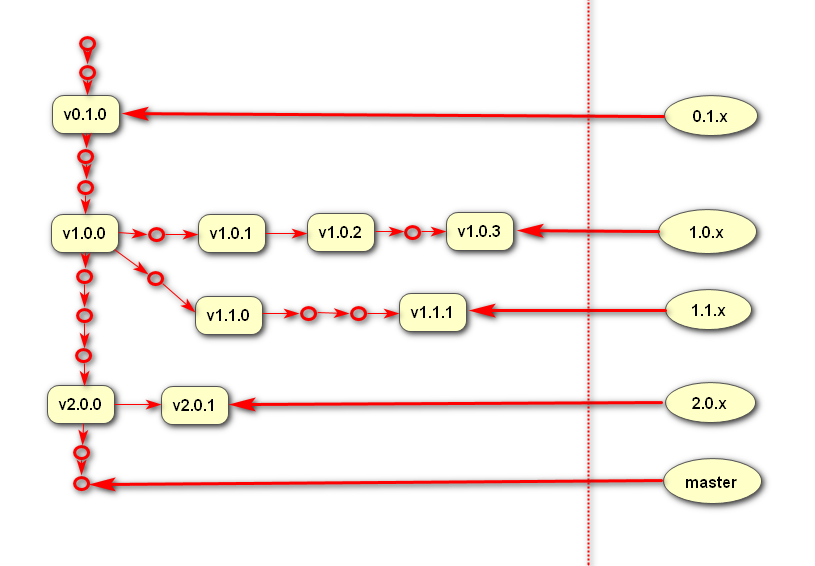
\includegraphics[width=\linewidth]{img/branches.png}
		\caption{Esempio di versionamento tramite l'utilizzo di \textit{branch}}
		\label{fig:branches}
	\end{figure}

	Quando si lavora su una repository condivisa è utile inoltre utilizzare i \textit{branch}, ovvero linee di sviluppo indipendenti che non vanno a interferire con il software in produzione.
	Tali branch possono essere utilizzati da una sola persona in maniera da non interferire con il lavoro di altri o da un team di persone.
	Nel caso in cui vi fossero errori nel branch, questi possono essere corretti senza che il resto del sistema ne sia influenzato.
	Ulteriormente, tali branch possono essere cancellati senza che il resto del sistema ne sia colpito.
	
	La Fig. \ref{fig:branches}~rappresenta sulla sinistra la linea di sviluppo tramite commit e branch mentre sulla destra le versioni attuali del sistema.
	
	Per i CI che rappresentano una versione MAJOR di una porzione di software, verrà utilizzato l'approccio \textit{PUSH}, ovvero la nuova versione viene mandata a tutti gli utilizzatori del sistema che dovranno installarla (a meno che l'installazione non avvenga automaticamente).
	Le versioni MINOR e PATCH verranno rilasciate secondo l'approccio \textit{PULL}, ovvero saranno gli utilizzatori del sistema a decidere il momento in cui effettuare il download e l'update alla nuova versione.
	In certi casi, come ad esempio il fix di un bug che compromette la sicurezza del sistema, queste potranno tuttavia essere rilasciate in modalità PUSH, obbligando dunque a installare subito la nuova versione.
	
%	Questa sezione descrive la gestione della configurazione da seguire durante l’implemen-
%	tazione del progetto.
%	Nonostante un’analisi approfondita della gestione della configurazione, scopo del
%	processo di Service Asset and Configuration Management, esuli dagli scopi di
%	questo documento, l’Offerente ritiene utile presentare le metodologie e le convenzioni
%	di massima che intende seguire durante il rollout.
%	Ricordiamo che l’obiettivo del Configuration Management è di fornire un modello
%	logico dell’infrastruttura attraverso l’identificazione, il controllo, la gestione e la verifica
%	di tutte le versioni dei Configuration Items (CI) esistenti. Un CI è un’unità strutturale
%	fondamentale di un sistema di gestione della configurazione. Alcuni esempi di CI sono:
%	documenti, software e componenti hardware. I CI sono memorizzati all’interno di un
%	database, detto CMDB.
%	Per garantire la possibilità di identificazione univoca, ogni CI sarà identificato da:
%	∗ ID: identificativo univoco.
%	∗ Numero di versione: numero nella forma X.Y.Z che segue le norme del
%	Semantic Versioning (https://semver.org/). In particolare
%	– X: numero di versione major, che indica un cambiamento radicale e
%	incompatibile con le versioni precedenti del CI.
%	– Y: numero di versione minor, che indica un’aggiunta di funzionalità al CI
%	compatibile con le versione precedenti.
%	– Z: numero di versione patch/emergency, che indica una risoluzione di
%	problemi del CI compatibile con le versioni precedenti.
%	Il numero di versione major 0 dev’essere utilizzato per i CI durante lo sviluppo iniziale.
%	Dopo il go-live, i CI assumono numero di versione 1.0.0.
%	L’Offerente prevede di rilasciare le major release esclusivamente con un approccio
%	push. Questo approccio prevede che l’azione di ricevimento/installazione della release
%	parta centralmente, avviata da parte dell’Offerente. Questa scelta è dovuta al fatto che
%	le major release non sono retrocompatibili e l’Offerente reputa che la gestione di due o
%	più CI con associate due major release diversi potrebbe essere fonte di inefficienze.
%	Per quanto riguarda le minor e le patch/emergency release verranno rilasciate con un
%	approccio pull+push. Questo approccio consiste nel rendere disponibile una release
%	centralmente e permettere agli utenti di applicarla on-demand quando lo ritengono
%	necessario. Tuttavia, dato che non c’è garanzia alcuna sul fatto che gli utenti prelevino
%	la release, l’Offerente si occuperà di rilasciare la release in modalità push dopo un certo
%	limite di tempo, di norma una settimana ma variabile in base alla gravità e all’urgenza
%	della release. Così facendo si uniscono i vantaggi della modalità push (rilasciare una
%	release a tutti) a quella pull (dare la possibilità all’utente di scegliere il momento più
%	opportuno per l’installazione).
	
\newpage
\section{Pianificazione dell'implementazione}\label{sec:pianificazione}

	Vengono quindi presentati in questa sezione alcuni diagrammi di Gantt che fungono come rappresentazione della pianificazone temporale del progetto e delle milestone.
	Per ciascuna attività vengono assegnate una \textit{data di inizio}, una \textit{data di fine} e una \textit{durata}.
	Si suppone che la firma del contratto e l'inizio del lavoro avvengano in data 1 Febbraio 2021.
	
	
	
	% Questi diagrammi sono stati creati tramite il software \textit{Gantt Project}\cite{gantt_project}.
	
\newpage
\section{\rollback~del sistema}

	% https://everythingwhat.com/what-is-a-rollback-plan-in-change-management
	% A rollback plan is exactly what it sounds like. It's a list of steps you'd take to undo a release and restore the system to its original state. Writing a rollback plan can also help clarify what impact the release is expected to have on other systems and what other steps should be taken.

	Avere un piano di \rollback~è essenziale quando si pianifica l'implementazione di una nuova feature all'interno di un sistema.
	È quindi composto da una lista di passi da seguire per disfare o annullare quello che è stato introdotto, andando quindi a ripristinare il sistema al suo stato originario.
	
	Un piano di \rollback~ben definito può aiutare inoltre a chiarificare l'impatto che un upgrade o l'installazione di una nuova release ha sul sistema e in che modo questo ne viene influenzato.

	È quindi necessario creare un piano di \rollback~per ciascuna nuova versione del sistema.
	A questo scopo verranno messi a disposizione da \azienda~alcuni template della documentazione necessaria per fissare i passi da seguire in caso di \rollback.
	Questi variano in base al tipo di installazione che si viene a eseguire, ovvero in caso venga installato semplicemente una \textit{patch}, una \textit{minor release} o una \textit{major release}, come descritte in \ref{sec:configurazione}.
	
%\section{Impatto dell'implementazione}
%
%	\subsection{Impatto sugli utenti}
%	\subsection{Impatto sui pazienti}
%	\subsection{Impatto sulla rete}
%	\subsection{Impatto sugli SLA}
%
%\newpage
%\section{Gestione andamento del progetto}
%
%	In questa sezione sono descritte le tecniche per il monitoraggio dello sviluppo del progetto in maniera da garantire un'implementazione \textit{efficiente} ed \textit{efficace}.
%	Tali controlli sono  essenziali per poter garantire che \azienda~sta procedendo nella giusta direzione e soddisfa i requisiti posti dall'istituto e, in caso contrario, procedere a correggere tempestivamente le situazioni di errore.
%	
%	Per poter controllare l'avanzamento del progetto sono dunque necessari dei parametri e delle metriche oggettive per la valutazione delle performance.
%	\'E importante quantificare il raggiungimento di certi obiettivi.
%
%	Per ciascuna metriche presenti in questa sezione e che \azienda~ha deciso di utilizzare, verranno assegnati dei criteri quali \textit{accettabilità} ed \textit{ottimalità}, con il seguente significato:
%	\begin{itemize}
%		\item \textit{accettabilità}: tale valore rappresenta una metrica accettabile e che non ha ancora raggiunto il livello ottimale, questo implica il dover continuare a lavorarci sopra;
%		\item \textit{ottimalità}: indica che la metrica misurata ha raggiunto un valore ottimale e che quindi l'obiettivo che sta misurando risulta pienamente soddisfatto.
%	\end{itemize}
%
%	Nel caso in cui vi siano valori esterni ai range indicati, allora la metrica misurata risulta ancora non accettabile.
%
%	\newpage
%	\subsection{Soddisfazione del Proponente}
%			
%		\azienda~ha deciso che questa metrica verrà misurata tramite meeting quindicinnali che possano dare feedback relativi all'avanzamento del lavoro.
%		
%		In ciascuno di questi meeting, gli stakeholder verranno messi a conoscenza dello stato di avanzamento del progetto, delle milestone raggiunte, di quelle prossime al raggiungimento e delle modifiche effettuate.
%		
%		Successivamente verranno raccolti i pareri degli stakeholders tramite questionari e testimonianze vocali, quando non risultano all'interno delle domande chieste nel questionario.
%		
%		Per ciascuno di questi verrà svolto un lavoro di analisi che indicherà quanto sono soddisfatti gli stakeholders.
%		
%		\begin{itemize}[noitemsep]
%			\item \textit{Range}: 1 - 10;
%			\item \textit{Range di accettabilità}: 6 - 8, indica che il lavoro sta procedendo nella direzione giusta, ma non è ancora soddisfacente;
%			\item \textit{Range di ottimalità}: 9 - 10, indica che il lavoro è arrivato al termine e soddisfa pienamente gli stakeholders.
%		\end{itemize}
%		
%		
%		
%	\newpage
%	\subsection{Tempismo nell’esecuzione dei lavori}
%	
%%		Le rilevazioni sul tempismo verranno effettuate ogni due settimane, in coincidenza
%%		con la redazione della documentazione di avanzamento progetto da parte dei membri
%%		del team dell’Offerente.
%	
%	\newpage
%	\subsection{Rispetto del budget}
%	
%%		Dato che la gestione del budget è legata intrinsecamente ad altre variabili,
%%		come qualità, portata e produttività, tenerla sotto controllo è fondamentale per il
%%		successo del progetto.
%%		Le rilevazioni sul budget verranno effettuate, come per la metrica precedente, ogni
%%		due settimane. Verranno indicate come scostamento percentuale rispetto al budget
%%		pianificato per quel periodo
%	
%	\newpage
%	\subsection{Rispetto degli SLA}
%		
%%		Concentrarsi esclusivamente sull’imple-
%%		mentazione della nuova soluzione e tralasciare la fornitura di servizi di qualità non è
%%		accettabile.
%%		Le rilevazioni per questa metrica verranno effettuate mensilmente, anche se il
%%		periodo di osservazione per gli SLA identificato nel capitolato risulta essere di 4 mesi.
%%		L’Offerente ritiene che misurare con questa frequenza possa dare risultati più tempestivi
%%		durante la fase di implementazione.
%	
%	\newpage
%	\subsection{Risolvimento incidenti al primo livello}
%	
%%		La rilevazione verrà effettuata su base mensile per tenere sotto controllo le perfor-
%%		mance del Service Desk.
%	
%\newpage
%\section{Livelli di servizio garantiti}

%
%livelli di servizio garantiti, partendo da quelli minimi indicati nel presente Capitolato Tecnico;
%3. la presa in carico degli attuali sistemi fino alla loro sostituzione, secondo la proposta progettuale dell’offerente, o il mantenimento ed adeguamento degli stessi nel rispetto dei
%la presa in carico degli attuali sistemi fino alla loro sostituzione, secondo la proposta progettuale dell’offerente, o il mantenimento ed adeguamento degli stessi nel rispetto dei requisiti e dei livelli di servizio definiti nel presente Capitolato Tecnico;
%progettuale dell’offerente, o il mantenimento ed adeguamento degli stessi nel rispetto dei requisiti e dei livelli di servizio definiti nel presente Capitolato Tecnico;

%\newpage
\section{Criteri di accettazione}

	Per ciascuna attività, come quelle descritte in Sez. \ref{sec:attivita_principali}, vi sono alcuni \textit{criteri di accettazione} che ne decretano la corretta conclusione.

	Secondo il framework ITIL, l'accettazione (o \textit{validazione}) viene eseguita dal processo di \textit{Service Validation and Testing}, composto dai seguenti sottoprocessi:
	% TODO cambiare
	\begin{itemize}[noitemsep]
		\item \textit{Definizione del modello di test} (o \textit{Test Model Definition}): specifica in dettaglio come la release verrà testata, definendo i test case da utilizzare per la validazione; 
		\item \textit{Acquisizione delle componenti della release} (o \textit{Release Component Acquisition}): acquisisce le componenti di una release e valuta inizialmente, assicurandosi che solo le componenti che superano dei controlli di qualità stringenti possano essere testate in modo intensivo;
		\item \textit{Test della release} (o \textit{Release Test}): testa tutte le componenti e tutti gli strumenti e le tecniche richieste per l’implementazione, la migrazione e il back out di una release. Solo le componenti che superano questi test possono entrare nell’ambiente live;
		\item \textit{Test di accettazione del servizio} (o \textit{Service Acceptance Testing}): verifica che sussistano tutte le condizioni affinchè il servizio possa essere attivato e ottiene il consenso da parte dell’utente che il servizio rispetta gli SLA concordati.
	\end{itemize}
	
	\begin{figure}[h!]
		\centering
		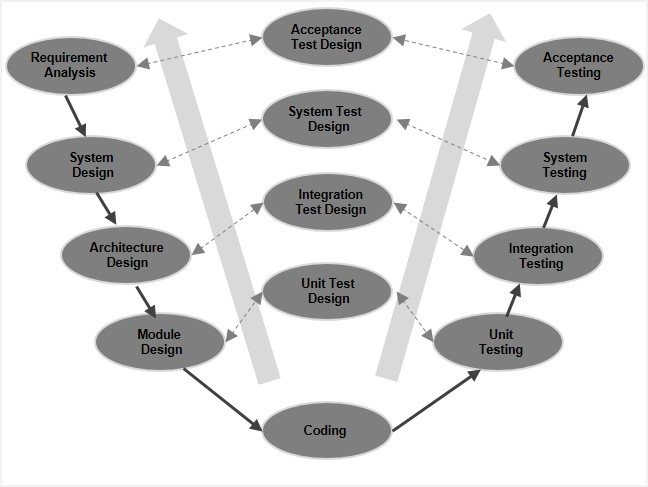
\includegraphics[width=\linewidth-2cm]{img/sdlc_v_model.jpeg}
		\caption{Modello a V\cite{vmodel}}
		\label{fig:vmodel}
	\end{figure}

	\azienda, come per altri progetti svolti in passato, ritiene opportuno utilizzare il ``\textit{Modello a V}'', rappresentato in Fig. \ref{fig:vmodel}, come approccio per la Verifica e Validazione.
	
	La validazione esterna, ovvero quella svolta attraverso i test di sistema insieme al propontente, è di importanza cruciale per \azienda.
	Per questo motivo viene data particolare attenzione a questi in quanto step finale per certificare la conformità complessiva del progetto.
	
	Tuttavia questa situazione non dovrebbe accadere in quanto verranno pianificati meeting quindicinnali insieme agli stakeholders per validare l'andamento del progetto.
	L'esito di tali meeting verrà salvato in documenti che conterranno i punti che sono stati trattati e gli interventi delle persone coinvolte.

\newpage
\section{Gestione dei rischi ed impatto}\label{sec:rischi}

	In questa sezione viene descritto come verranno catalogati i rischi ed i problemi che possono provocare danni al sistema, alle informazioni che questo contiene e, dunque, ai pazienti e ai dipendenti che lo utilizzano.
	
	Secondo il \textit{CRAMM} (``\textit{CCTA Risk Analysis and Management Method}''), il rischio si può definire come il prodotto tra valore dell'asset, minaccia e vulnerabilità.
	
	\begin{figure}[h!]
		\centering
		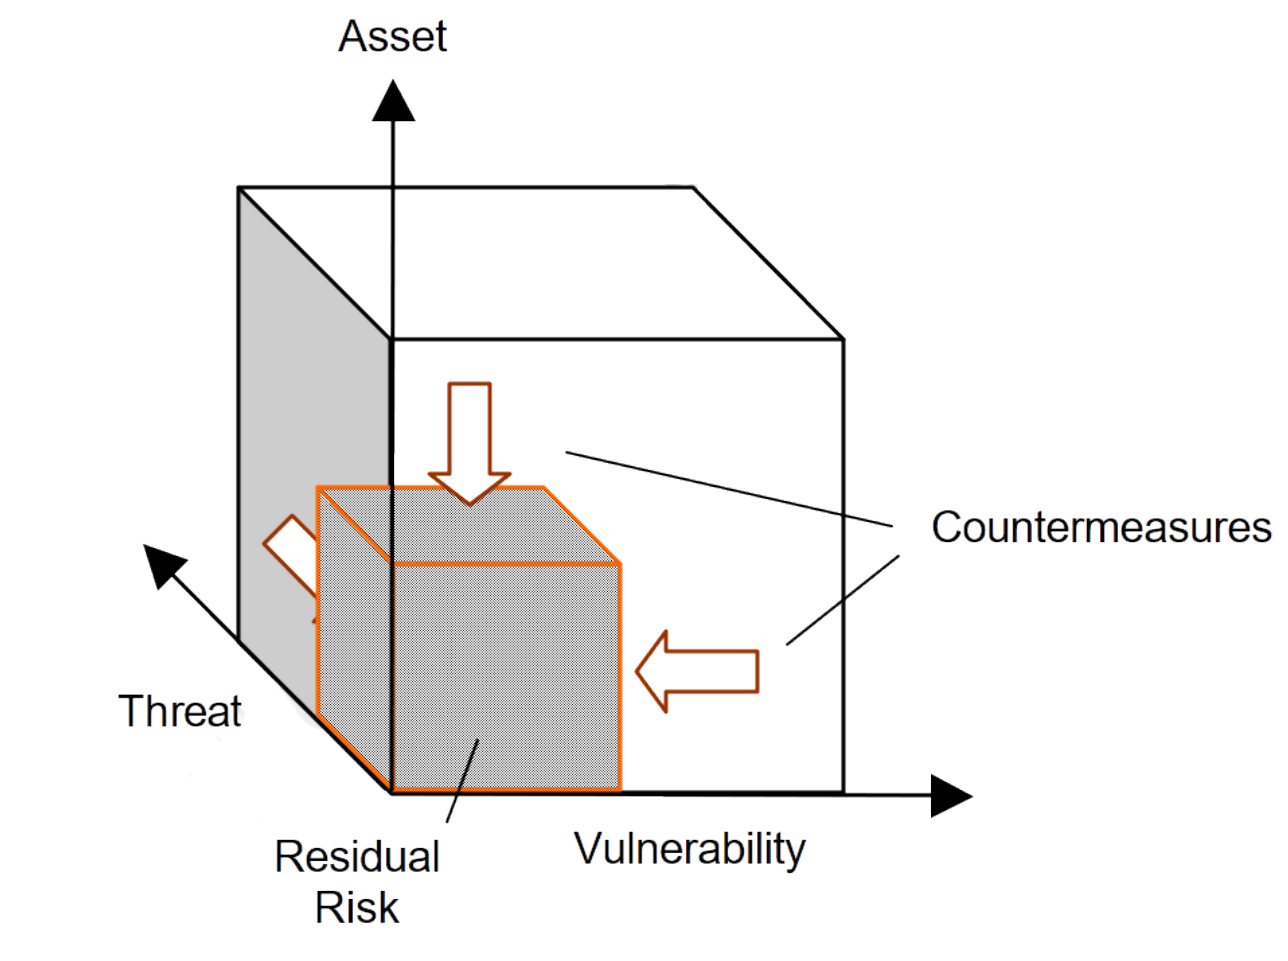
\includegraphics[width=\linewidth-2cm]{img/risk.png}
		\caption{Rappresentazione del rischio\cite{risk}}
		\label{fig:risk}
	\end{figure}

	Per stimare l'impatto dei rischi viene utilizzata la matrice ``\textit{probabilità-impatto}'' rappresentata in Fig. \ref{fig:risk_matrix}, dove livello di rischio viene calcolato come l'intersezione tra:
	\begin{itemize}[noitemsep]
		\item \textit{Probabilità}: la risposta alla domanda ``\textit{quanto è probabile che accada questo evento?}'';
		\item \textit{Impatto}: la risposta alla domanda ``\textit{quanto è sconvolgente questo evento sul sistema?}'';
	\end{itemize}
	Il rischio ha quindi una misura qualitativa che può avere questi valori:
	\begin{itemize}[noitemsep]
		\item \textit{Rischio molto basso}: tale evento ha un impatto minimo sul sistema e sui suoi utenti, è possibile rivolgerlo nella versione da rilasciare successivamente;
		\item \textit{Rischio basso}: tale evento può provocare sconforto nell'uso del sistema da parte degli utenti;
		\item \textit{Rischio moderato}: tale evento può risultare in un downtime del sistema e necessita di essere analizzato con cura;
		\item \textit{Rischio alto}: tale evento minaccia il sistema e deve essere risolto prima che accada;
		\item \textit{Rischio molto alto}: tale evento mette a repentaglio la sicurezza del sistema e dei suoi utenti risultando catastrofico per l'\istituto. 
		Va risolto immediatamente e tutto il sistema va aggiornato.
	\end{itemize}
	
	\begin{figure}[h!]
		\centering
		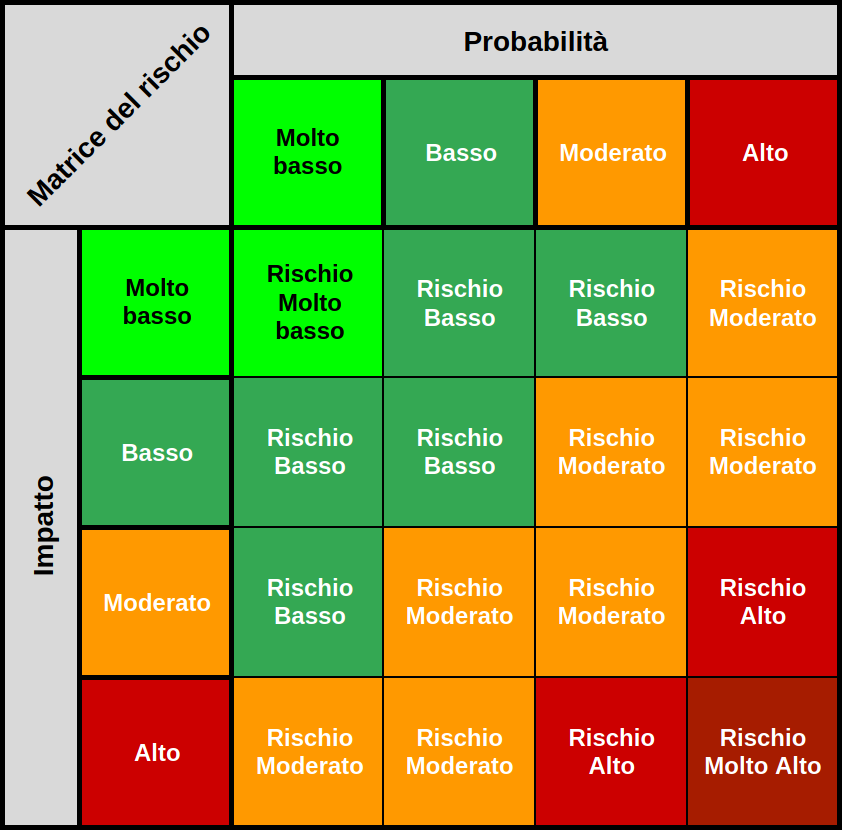
\includegraphics[width=\linewidth]{img/matrix.png}
		\caption{\textit{Risk Assessment Matrix}}
		\label{fig:risk_matrix}
	\end{figure}

	Un'analisi approfondita dei rischi sarà presentata nella documentazione riguardante il processo di ``\textit{Risk Management}''.

\newpage
\section{Privacy e sicurezza del sistema}

	\azienda~si impegna a garantire che il progetto svolto per l'\istituto~sia sicuro considerando gli standard della privacy e quelli della sicurezza.
	Per questo tali aspetti verranno trattati durante l'implementazione seguendo i principi di \textit{security by design}.

	\subsection{Privacy}
		
		Per tale aspetto, il regolamento principale su cui fare affidamento è quello del 
		``\textit{General Data Protection Regulation}'' (o \textit{GDPR}), rilasciato nella prima metà del 2018.
		Seguendo questo regolamento ci sono due aspetti fondamentali da considerare:
		\begin{itemize}
			
			\item il primo riguarda il consenso del soggetto di cui si stanno trattando i dati. 
			Questo deve essere sempre richiesto preventivamente e senza che possa essere equivoco;
			escludendo ogni ipotesi di consenso tacito.
			
			\item il secondo riguarda i casi di violazioni esterne (o ``\textit{data breach}'') quali furti di informazioni via Internet o fisicamente.
			Se dovesse presentarsi questa situazione, il responsabile del sistema, in quanto titolare del trattamento dei dati, dovrà preoccuparsi di communicare l'accaduto immediatamente ai proprietari dei dati e ad eventuali soggetti come ad esempio il garante nazionale o la polizia postale.
			
		\end{itemize}
		
	\subsection{Sicurezza}
	
		Al di là della privacy dei dati e dei processi, è necessario che il sistema sia sicuro da ogni altra prospettiva.
		Dal punto di vista \textit{ITIL}, la sicurezza (\textit{security}) è:
		\begin{itemize}[noitemsep]
			\item \textit{Confidentiality};
			\item \textit{Integrity};
			\item \textit{Availability}.
		\end{itemize}
	
		Questi tre componenti, che formano l'anagramma di \textit{CIA}, rispondono alle violazioni  del sistema con contenimenti e correzioni.
		
		I livelli di security che vengono descritti da ITIL si basano principalmente in ambito IT, ovvero sugli strumenti e sulle tecnologie, a differenza della privacy che ha un maggiore orientamento verso i processi.
  	\chapter{Attività e risorse di supporto}\label{ch:supporto}

In questo capitolo vengono descritte le attività ed altre risorse considerate secondarie e di supporto all'implementazione del nuovo sistema informatico dell'\istituto.

Tali risorse possono essere di natura informatica, come hardware, software e altri materiali, o di natura aziendale come strutture, documenti, personale e requisiti di formazione.

\section{Documentazione}

	Per poter illustrare correttamente il nuovo sistema e l'implementazione dell'intero progetto, \azienda~produrrà documenti quali:
	\begin{itemize}[noitemsep]
		
		\item \textit{Composizione dei Processi Aziendali}: contiene l'analisi del vecchio sistema gerarchico, la transizione ai nuovi BPR e una descrizione dettagliata di questi;
		
		\item \textit{Analisi e architettura della rete e dei sistemi interni}: contiene un'analisi del vecchio sistema informatico a livello architetturale e di rete, la descrizione dettagliata della nuova rete, inclusiva dell'hardware utilizzato e delle postazioni dei dipendenti, del piano di indirizzamento IP e del partizionamento della nuova rete;

		\item \textit{Documento di avanzamento dei lavori}: questo documento conterrà tutti i rapporti redatti riguardanti l'avanzamento dei lavori;
		
		\item \textit{Documentazione relativa ai test}: tale documento conterrà tutte le informazioni necessarie per quanto riguarda i test (da \textit{unit test} a \textit{test di accettazione}) svolti sul sistema e che possono essere rifatti a cadenza temporale, oppure svolti per particolari eventi, come, per esempio, la release e l'implementazione di una nuova feature.
		Una porzione di questo documento può essere dedicata ai rischi, descrivendoli come specificato in \ref{sec:rischi}, a come evitarli o mitigarli e a quali test sono stati eseguiti per poterli prevenire;
		
		\newpage
		\item \textit{Documento aggiornato dei ``progetti innovativi''}: vista la richiesta dell'\istituto~di lavorare su progetti innovativi, è necessario tenere traccia di questi in un documento che sia in costante aggiornamento.
		Tale documento conterrà la descrizione di ciascun progetto attraverso l'uso di template precedentemente concordati dai tecnici di \azienda~e dal \proponente, in base alle necessità di quest'ultimo.
		
	\end{itemize}

	Tali documenti serviranno non solamente ai futuri tecnici dell'\istituto~per capire il funzionamento del sistema, ma anche agli stakeholders, che, tramite tali elaborati, potranno seguire l'avanzamento del progetto.

\section{Materiale informatico}

	Tutto il materiale informatico e relativa documentazione che l'\istituto~possiede dovrà essere messa a disposizione ai dipendenti di \azienda~per poter garantire che tutti i servizi attualmente erogati siano noti durante la transizione e che questi possano essere replicati nel nuovo sistema.

	\subsection{Hardware}
		
		Come specificato dal \proponente~nel capitolato, tutto l'hardware dell'attuale sistema sarà preso in carica dall'\offerente.
		Questo include tutta l'infrastruttura tecnologica specificata dall'\istituto~nel capitolato.
		
	\subsection{Software}
	
		Come per l'hardware, anche il software verrà preso in carica dal \offerente.
		I sistemi applicativi di tutte le aree verranno messe a disposizione ad \azienda, la quale si prenderà cura di mantenerli attivi durante la transizione e di effettuare backup periodici, completi o incrementali, in caso fosse necessario effettuare un \rollback.
	
\section{Strutture}

	Per la corretta installazione del nuovo sistema informatico, e, di conseguenza, il corretto completamento del progetto, è necessario l'accesso alle strutture ospedaliere.
	Questo implica una concessione periodica, valida dall'inizio del progetto, di credenziali e di permessi di accesso da parte del \proponente~ad \azienda~per poter permettere ai suoi dipendenti di entrare e uscire dagli edifici che compongono l'\istituto.

\section{Personale}

	Anche il personale messo a disposizione dall'\istituto~rappresenta un asset importante per il corretto svolgimento del progetto.
	
	\subsection{Requisiti di staff}
	
		Per implementare correttamente il progetto non sforando il tempo e il budget prefissati, \azienda~necessita che l'\istituto~metta a disposizione i propri dipendenti di varie aree.
		
		\azienda, per riuscire a creare una piattaforma ad hoc, necessita di avere feedback non solamente dai principali stakeholders, ma anche da coloro che la useranno giornalmente.
		Per questo inizialmente verranno somministrati alcuni questionari, non soltanto riguardo le feature più utilizzate, ma anche sull'interfaccia grafica più adatta all'utilizzo dei dipendenti.
		
		I tecnici dell'\istituto~verranno affiancati dai dipendenti di \azienda~per trovare la soluzione migliore ai bisogni presentati all'interno del capitolato.
	
	\subsection{Formazione dello staff}
	
		La formazione dello staff dell'\istituto~da parte di \azienda~è uno step principale per quanto riguarda la fase di riconsegna del progetto.
		Senza un corretto corso di formazione ed un sufficente affiancamento, il personale dell'\istituto~non sarà in grado di utilizzare correttamente i nuovi strumenti sviluppati appositamente da \azienda.
	
		\subsubsection{Formazione tecnica}
			
			Questa riguarda lo staff che sarà a stretto contatto con il nuovo sistema di \helpdesk~e che dovrà rispondere efficacemente alle richieste degli utenti, agendo da \textit{single point of contact}, come spiegato in \ref{sec:scopo_helpdesk}.
		
			Tale personale deve essere esperto in materia informatica, avendo preferibilmente una certificazione in \textit{ITIL Foundations}.
			La conoscenza dei processi ITIL permette ai dipendenti di poter capire a fondo come è strutturato il nuovo sistema e come poter intevenire professionalmente in caso di bisogno.
			
			I dipendenti sottoposti alla formazione tecnica dovranno avere una profonda conoscenza del processo di Business Process Reengineering, e verranno sottoposti a test di valutazione, sia in fase di presa in carico sia prima della conclusione del BPR, per verificare la corretta comprensione dei nuovi processi aziendali.
			
			Il personale continuerà ad essere formato anche dopo la riconsegna del progetto: verranno calendarizzate sessioni regolari di formazione per poter permettere ai dipendenti di imparare il nuovo sistema e ad essere pratici dei nuovi processi.
			
			Tali sessioni di aggiornamento possono essere tenute nel normale orario di lavoro, ma, per garantire una corretta e continuativa erogazione dei servizi di Service Desk, ne verranno proposte di più (due o tre) alle quali i dipendenti potranno aderire.
			
		\subsubsection{Formazione non tecnica}
			
			In aggiunta alla formazione del personale a stretto contatto con le tecnologie e con l'architettura del \helpdesk, vi è anche un training per i dipendenti dell'\istituto~che non fanno parte dei tecnici.
			
			A tale staff verrà effettuata una completa formazione sulla nuova interfaccia del sistema, sulle nuove funzionalità che sono state aggiunte e sui nuovi metodi per contattare il Service Desk in caso di bisogno.
			
			Oltre alla formazione iniziale, che verrà effettuata dai dipendenti di \azienda~presso la sede dell'\istituto, verranno forniti ai dipendenti tutti i documenti e i manuali, non tecnici, che sono stati redatti durante lo svolgimento del progetto e che possono essere di aiuto in caso di studio personale.
			
			Come per la formazione tecnica, anche per questo tipo di formazione è necessario un corso di aggiornamento, in questo specifico caso a cadenza minore.
			Le date e la frequenza di queste sessioni verranno concordate successivamente tra \azienda~e l'\istituto.
		
	
    \include{sez/contatti}

    \begin{thebibliography}{9}

\bibitem{istituto} 
	Sito ufficiale dell'\textit{Istituto Ortopedico Gaetano Pini}:\\
	\url{https://www.asst-pini-cto.it/}
	
\bibitem{sito_azienda}
	Sito ufficiale di \textit{\azienda}:\\
	\url{https://www.linkedin.com/in/cvoinea/}

\bibitem{itil_website}
	Sito ufficiale di \textit{AXELOS}:\\
	\url{https://www.axelos.com/best-practice-solutions/itil}

\bibitem{release_deployment_management}
	\textit{Release and Deployment Management}:\\
	\url{https://wiki.en.it-processmaps.com/index.php/Release_and_Deployment_Management}

\bibitem{service_desk}
	\textit{ITIL Service Desk types}:\\
	\url{https://advisera.com/20000academy/blog/2014/05/06/itil-service-desk-types/}
	
\bibitem{bpr}
	\textit{Business process re-engineering}:\\
	\url{https://en.wikipedia.org/wiki/Business_process_re-engineering}
	
%\bibitem{gantt_project}
%	\textit{Gantt Project official website}:\\
%	\url{https://www.ganttproject.biz/}

\bibitem{github}
	Sito ufficiale di \textit{GitHub}:\\
	\url{https://github.com/}

\bibitem{bitbucket}
	Sito ufficiale di \textit{BitBucket}:\\
	\url{https://bitbucket.org/product}

\bibitem{gitlab}
	Sito ufficiale di \textit{GitLab}:\\
	\url{https://about.gitlab.com/}
	
\bibitem{semantic}
	Sito ufficiale di \textit{Semantic Versioning}:\\
	\url{https://semver.org/}
	
\bibitem{vmodel}
	\textit{SDLC - V-Model}:\\
	\url{https://www.tutorialspoint.com/sdlc/sdlc_v_model.htm}

\bibitem{risk}
	\textit{SANS InstituteInformation Security Reading Room}:\\
	\url{https://www.sans.org/reading-room/whitepapers/auditing/qualitative-risk-analysis-management-tool-cramm-83}


%\bibitem{latexcompanion} 
%Michel Goossens, Frank Mittelbach, and Alexander Samarin. 
%\textit{The \LaTeX\ Companion}. 
%Addison-Wesley, Reading, Massachusetts, 1993.
%
%\bibitem{einstein} 
%Albert Einstein. 
%\textit{Zur Elektrodynamik bewegter K{\"o}rper}. (German) 
%[\textit{On the electrodynamics of moving bodies}]. 
%Annalen der Physik, 322(10):891–921, 1905.
%
%\bibitem{knuthwebsite} 
%Knuth: Computers and Typesetting,
%\\\texttt{http://www-cs-faculty.stanford.edu/\~{}uno/abcde.html}
\end{thebibliography}
    
%    \appendix
      
%    \chapter{Timeline}\label{ch:appendice_a}
    

\end{document}